\documentclass[12pt,a4paper]{article}
\usepackage{ucebnice}

\title{Komplexní čísla}
\author{Ondřej Škubala}
\date{\today}
\begin{document}
\maketitle
\newpage





\begin{historicalbox}
Komplexní čísla patří mezi matematické objekty, jejichž vznik nebyl motivován pouze
snahou zavést nový druh čísel, ale především potřebou řešit rovnice, které tehdejší
číselné obory nedokázaly dostatečně popsat. Podobně jako záporná čísla vznikla
přirozeným rozšířením čísel kladných a racionální čísla umožnila vyjádřit podíly,
které nebylo možné zapsat pomocí celých čísel, vedl další rozvoj algebry k otázce,
zda lze nějakým smysluplným způsobem pracovat také s odmocninami záporných čísel.

První výraznější problémy tohoto typu se objevily v renesanční Itálii v souvislosti
s řešením rovnic třetího stupně. Italský matematik Gerolamo Cardano
(1501--1576) ve svém díle \textit{Ars Magna}, vydaném roku 1545, narazil při
algebraických výpočtech na výrazy obsahující odmocniny záporných čísel. Takové
výrazy působily velmi podivně, protože žádné tehdy známé číslo umocněné na druhou
nemohlo dát záporný výsledek, a proto nebylo zřejmé, zda mají tyto objekty vůbec
nějaký matematický význam.

Zásadní posun přinesl Rafael Bombelli (1526--1572), který ve svém díle
\textit{L'Algebra} z roku 1572 ukázal, že s odmocninami záporných čísel lze
počítat podle pevných pravidel a že jejich použití může vést ke zcela reálným
výsledkům. Právě tato skutečnost byla mimořádně důležitá, protože ukázala, že
podivné výrazy vznikající během výpočtu nemusí být matematickou chybou, nýbrž
mohou představovat nový druh čísel, který rozšiřuje dosavadní číselný systém.
René Descartes (1596--1650) použil roku 1637 ve svém díle
\textit{La Géométrie} pro tato čísla označení \emph{imaginární}. Název měl
původně vyjadřovat jejich poněkud problematické postavení, protože tato čísla nebylo
možné chápat jako běžné délky ani je umístit na tehdy používanou číselnou osu.
Pojmenování se však zachovalo a používáme je dodnes.

V 18. století začala být imaginární čísla běžnou součástí algebry a symbol
\[
    i
\]
se pro imaginární jednotku prosadil zejména díky Leonhardu Eulerovi (1707--1783).
Postupně se zároveň ukázalo, že tato čísla nejsou pouze formálním algebraickým
trikem, ale že mají také přirozený geometrický význam.

Caspar Wessel na konci 18. století a později Jean-Robert Argand ukázali, že komplexní
čísla lze zobrazovat jako body v rovině, přičemž Carl Friedrich Gauss tuto geometrickou
interpretaci dále rozvinul a výrazně přispěl k jejich všeobecnému přijetí.
Komplexní čísla se tak postupně změnila z původně podezřelých a
``imaginárních'' objektů v jeden ze základních číselných oborů moderní matematiky.
Dnes se používají nejen v samotné algebře a matematické analýze, ale také ve fyzice,
elektrotechnice, teorii signálů, kvantové mechanice či při studiu kmitání a vlnění.
\end{historicalbox}



\section{Imaginární jednotka}
Nejprve si pojďme připomenout úpravy jednoduchých rovnic, se kterými jsme se již setkali v předchozích kapitolách. Uvažujme například rovnici
\[
x+5=2.
\]
Pomocí běžné ekvivalentní úpravy odečteme od obou stran číslo \(5\):
\begin{align*}
    x+5 &= 2,\\
    x   &= 2-5,\\
    x   &= -3.
\end{align*}
Rovnice má tedy právě jedno řešení,
\[
K=\\{-3\\}.
\]
Správnost výsledku můžeme snadno ověřit dosazením:
\[
    -3+5=2,
\]
takže číslo $x=-3$ skutečně původní rovnici splňuje. Přestože je výsledek záporný, 
nepředstavuje pro nás žádný problém, protože pracujeme v oboru reálných čísel, 
který záporná čísla obsahuje.

Pojďme se nyní podívat na jinou, stále velmi jednoduchou rovnici:
\[
    x^2+1=0.
\]
Opět provedeme běžnou ekvivalentní úpravu a odečteme od obou stran číslo $1$:

\begin{align*}
x^2+1   &= 0,\\
x^2     &= -1.
\end{align*}

V tomto okamžiku však narazíme na problém. Hledáme takové číslo $x$, 
jehož druhá mocnina je rovna \(-1\), avšak pro každé reálné číslo platí
\[
    x^2\geq 0.
\]
Je-li $x>0$, je jeho druhá mocnina kladná; je-li $x<0$, 
násobíme při výpočtu $x^2=x\cdot x$ dvě záporná čísla, 
a výsledek je proto opět kladný. Pro $x=0$ samozřejmě dostáváme $x^2=0$.

Žádné reálné číslo tedy nemůže splňovat rovnost
\[
    x^2=-1.
\]
V oboru reálných čísel proto rovnice $x^2+1=0$ nemá žádné řešení a zapisujeme
\[
    K=\emptyset.
\]
Mohli bychom tímto výpočet ukončit a jednoduše prohlásit, 
že daná rovnice nemá v oboru reálných čísel řešení.
V matematice jsme se však s podobnou situací již několikrát setkali.

Rovnice
\[
    x+5=2
\]
by například neměla řešení, pokud bychom připouštěli pouze přirozená čísla, 
protože její řešení $x=-3$ do množiny $\mathbb{N}$ nepatří. 
Problém jsme však vyřešili rozšířením číselného oboru na čísla celá.
Podobnou myšlenku můžeme použít i nyní. Namísto toho, abychom rovnici
\[
    x^2=-1
\]
označili za definitivně neřešitelnou, rozšíříme znovu náš číselný obor
a zavedeme nový druh čísla, jehož druhá mocnina bude právě $-1$. 
Tím se dostáváme k pojmu \important{imaginární jednotky}.

\begin{definitionbox}
\textbf{Imaginární jednotkou} nazýváme číslo $i$, pro které platí
\[
    i^2=-1.
\]
\end{definitionbox}

V běžném zápisu se proto setkáváme také se vztahem
\[
    i=\sqrt{-1},
\]
přičemž základní definicí imaginární jednotky zůstává vztah $i^2=-1$.
Zavedením imaginární jednotky jsme nezměnili pravidla algebry, ale pouze jsme
rozšířili množinu objektů, se kterými můžeme tato pravidla používat. Podobný krok
jsme ostatně provedli již dříve při přechodu od přirozených čísel k celým, od celých
k racionálním a následně k reálným číslům.

Rovnice
\[
    x^2=-1
\]
proto již v novém číselném oboru řešení má. Protože podle definice platí
\[
    i^2=-1,
\]
je jedním řešením číslo \(i\). Zároveň však dostáváme
\[
    (-i)^2 = \left[(-1) \cdot i\right]^2 = (-1)^2 \cdot i^2 = 1 \cdot (-1) = -1,
\]
a druhým řešením je tedy číslo \(-i\).

Množinu řešení můžeme zapsat ve tvaru
\[
    K=\\{-i;i\\}.
\]
Tento jednoduchý příklad ukazuje, že zavedením imaginární jednotky dokážeme řešit
rovnice, které v oboru reálných čísel řešení nemají.


\subsection{Umocňování imaginární jednotky}
S imaginární jednotkou můžeme provádět běžné algebraické operace, přičemž musíme
respektovat její základní vlastnost $i^2=-1$.

Začneme poněkud netradičně umocňováním. Z definice imaginární jednotky vyplývá, že
\[
    i^2=-1.
\]
Když budeme pokračovat v umocňování, dostaneme
\[
    i^3=i^2\cdot i=(-1)\cdot i=-i,
\]
\[
    i^4=i^2\cdot i^2=(-1)(-1)=1.
\]
Kdybychom v umocňování pokračovali i dále
\[
    i^5=i^4\cdot i=1\cdot i=i,
\]
nebo
\[
    i^6=i^4\cdot i^2=1\cdot(-1)=-1,
\]
můžeme si všimnout, že se hodnoty mocnin imaginární jednotky pravidelně opakují.
Důvodem je vztah $i^4=1$, takže vynásobení libovolné mocniny číslem $i^4$
její hodnotu nezmění. Mocniny imaginární jednotky se proto opakují s periodou čtyři.

Z toho vyplývá, že pro každé celé nezáporné číslo \(n\) platí
\[
    i^{n+4}=i^n.
\]
Proto stačí znát pouze první čtyři mocniny imaginární jednotky, 
abychom mohli určit libovolnou vyšší mocninu.
\begin{align*}
    i   &= i    \\
    i^2 &= -1   \\
    i^3 &= -i   \\
    i^4 &= 1
\end{align*}

\begin{examplebox}
    Určete hodnoty $i^{20}$, $i^{42}$.

    \begin{minipage}[t]{0.48\textwidth}
        \[
        i^{20}  = i^4\cdot i^4 \cdot i^4 \cdot i^4 \cdot i^4
                = (i^4)^{5}
                = 1^{5}
                = 1
        \]
    \end{minipage}

    \begin{minipage}[t]{0.48\textwidth}
        \[
        i^{42}  = i^{40}\cdot i^2
                = (i^4)^{10}\cdot i^2
                = 1^{10}\cdot i^2
                = 1\cdot i^2
                = -1
        \]
    \end{minipage}

\end{examplebox}



\begin{notebox}

Při výpočtu vysokých mocnin imaginární jednotky není nutné číslo \(i\)

opakovaně násobit. Stačí určit zbytek exponentu po dělení čtyřmi (modulo 4).

Platí

\[
i^n=
\begin{cases}
    1,  & n\equiv 0 \pmod{4},\\
    i,  & n\equiv 1 \pmod{4},\\
    -1, & n\equiv 2 \pmod{4},\\
    -i, & n\equiv 3 \pmod{4}.
\end{cases}
\]

Pokud jsme se se zápisem kongruencí ještě nesetkali, stačí si z tohoto vztahu
zapamatovat jeho praktický význam: při určování mocniny $i^n$ rozhoduje pouze
zbytek exponentu $n$ po dělení čtyřmi.

\end{notebox}

\begin{examplebox}
    Určete hodnotu $i^{123}$.
    
    Číslo $123$ můžeme zapsat pomocí nejbližšího násobku čísla $4$:
    \[
        123 = 120 + 3
    \]

    Zbytek po dělení čtyřmi je tedy $3$, a proto
    \[
        i^{123}=i^3=-i.
    \]

\end{examplebox}

\begin{examplebox}
    Určete hodnotu $i^{2026}$.
    
    Exponent $2026$ vydělíme číslem $4$:
    \[
        2026 = 2024 + 2
    \]

    Při dělení čtyřmi tedy dostáváme zbytek $2$, a proto má $i^{2026}$ stejnou
    hodnotu jako \(i^2\):
    \[
        i^{2026}=i^2=-1.
    \]
\end{examplebox}







\section{Ryze imaginární čísla}
Jakmile máme k dispozici imaginární jednotku $i$, můžeme ji podobně jako běžná
čísla násobit libovolným reálným číslem. Vznikají tak například čísla
\[
    2i,
    \qquad
    -5i,
    \qquad
    \frac{3}{4}i,
    \qquad
    \sqrt{2}\\,i.
\]
Taková čísla nazýváme ryze imaginárními čísly. Jejich význam lze dobře
pozorovat při řešení rovnic, jejichž pravá strana je záporná.

Uvažujme například rovnici
\[
    x^2=-9.
\]
V oboru reálných čísel nemá tato rovnice řešení, protože druhá mocnina reálného
čísla nemůže být záporná. Po zavedení imaginární jednotky však můžeme záporné
číslo na pravé straně přepsat pomocí vztahu $i^2=-1$:

\begin{align*}
    x^2 &= -9,\\
    x^2 &= 9i^2,\\
    x^2 &= (3i)^2.
\end{align*}

Dostáváme tedy dvě řešení
\[
    x=\pm3i.
\]
Správnost obou kořenů můžeme snadno ověřit, protože platí
\[
    (3i)^2=9i^2=-9
\]
a také
\[
    (-3i)^2=9i^2=-9.
\]

\begin{definitionbox}
    \textbf{Ryze imaginárním číslem} nazýváme každé číslo tvaru
    \[
        bi, 
    \]
    kde $b\in\mathbb{R}; b\neq0$.
    Číslo \(b\) nazýváme koeficientem imaginární části.
\end{definitionbox}

Ryze imaginární čísla nám umožňují také zapisovat odmocniny záporných reálných
čísel. Je-li $a>0$, používáme zápis
\[
    \sqrt{-a}=i\sqrt{a}.
\]

Například
\[
    \sqrt{-4}=2i,
    \qquad
    \sqrt{-25}=5i,
    \qquad
    \sqrt{-2}=i\sqrt{2}.
\]

Je však důležité rozlišovat mezi symbolem odmocniny a řešením rovnice. Zápis
\[
    \sqrt{-9}=3i
\]

označuje zvolenou odmocninu čísla $-9$, zatímco rovnice
\[
    x^2=-9
\]

má dvě řešení
\[
    x=\pm3i.
\]

\begin{notebox}

Základním vztahem pro imaginární jednotku je

\[
    i^2=-1.
\]

Při práci s komplexními čísly proto není vhodné bez dalšího přenášet všechna
pravidla známá pro odmocniny nezáporných reálných čísel. Zejména vztah

\[
    \sqrt{uv}=\sqrt{u}\sqrt{v}
\]

nelze obecně používat pro libovolná komplexní čísla $u$ a $v$.
\end{notebox}

\subsection{Základní operace s imaginárními čísly}
S imaginárními čísly můžeme provádět stejné základní algebraické operace jako
s běžnými číselnými výrazy. Při sčítání a odčítání pracujeme s imaginární
jednotkou $i$ podobně jako s proměnnou, takže můžeme sčítat nebo odčítat její
koeficienty. Při násobení a dělení však navíc využíváme základní vlastnost
\[
    i^2=-1.
\]

Díky tomu nemusí být výsledkem operace dvou ryze imaginárních čísel opět ryze imaginární číslo;
například součin dvou imaginárních jednotek je číslo reálné.

\begin{examplebox}
    Proveďte následující operace s imaginárními čísly.

    \textbf{a) Sčítání}
    \[
        3i+5i.
    \]

    Protože oba členy obsahují stejnou imaginární jednotku $i$, sečteme jejich koeficienty:
    \begin{align*}
        3i+5i
        &= (3+5)i = 8i.
    \end{align*}

    \textbf{b) Odčítání}
    \[
        7i-12i.
    \]

    Stejným způsobem odečteme koeficienty:
    \begin{align*}
        7i-12i
        &= (7-12)i = -5i.
    \end{align*}

    \textbf{c) Násobení}
    \[
        (3i)(-4i).
    \]

    Nejprve vynásobíme reálné koeficienty a následně imaginární jednotky:
    \begin{align*}
        (3i)(-4i)
        &= 3\cdot(-4)\cdot i^2 \\
        &= -12\cdot(-1) \\
        &= 12.
    \end{align*}

    Vidíme tedy, že součin dvou ryze imaginárních čísel může být číslem

    reálným.

    \textbf{d) Dělení}

    \[
        \frac{12i}{3i}.
    \]

    Protože $i\neq0$, můžeme imaginární jednotku v čitateli a jmenovateli

    zkrátit:

    \begin{align*}
        \frac{12i}{3i}
        &= \frac{12}{3}\cdot\frac{i}{i} \\
        &= 4\cdot1 \\
        &= 4.
    \end{align*}

    Také podílem dvou nenulových ryze imaginárních čísel tedy může být

    reálné číslo.

    \textbf{e) Kombinace operací}

    \[
        \frac{(5i-2i)(i^3+3i)}{2i\cdot i^3}
        -
        \frac{6i}{3i}.
    \]

    Nejprve upravíme mocniny imaginární jednotky a výrazy v závorkách:

    \begin{align*}
        \frac{(5i-2i)(i^3+3i)}{2i\cdot i^3}
        -
        \frac{6i}{3i}
        &=
        \frac{3i(-i+3i)}{2i\cdot(-i)}
        -
        2
        \\[2mm]
        &=
        \frac{3i\cdot2i}{-2i^2}
        -
        2
        \\[2mm]
        &=
        \frac{6i^2}{-2i^2}
        -
        2
        \\[2mm]
        &=
        \frac{-6}{2}
        -
        2
        \\[2mm]
        &=
        -3-2
        \\[2mm]
        &=
        -5.
    \end{align*}

    Přestože původní výraz obsahoval pouze imaginární čísla, po provedení všech

    operací jsme získali číslo reálné.

\end{examplebox}





% ==================================================
% ================ KOMPLEXNÍ ČÍSLA =================
% ==================================================

\section{Komplexní čísla}
Doposud jsme pracovali jednak s reálnými čísly, 
se kterými jsme se setkávali v předchozích kapitolách, 
a jednak s nově zavedenými ryze imaginárními čísly.
Máme tedy například reálná čísla
\[
    3,\qquad -\frac{1}{2},\qquad \sqrt{2},\qquad \pi,
\]

a ryze imaginární čísla
\[
    2i,\qquad -5i,\qquad \frac{3}{4}i.
\]

Přirozeně se nyní nabízí otázka, co dostaneme, pokud reálné 
a imaginární číslo spojíme pomocí sčítání. Uvažujme například výraz
\[
    3+2i.
\]

Tento výraz již není reálným číslem, protože obsahuje imaginární jednotku $i$,
zároveň však není ani ryze imaginárním číslem, protože obsahuje nenulovou reálnou část.
Dostáváme tak nový druh čísla, které v sobě současně obsahuje část reálnou a část imaginární.
Taková čísla nazýváme \important{komplexní čísla}.

\begin{definitionbox}
    \textbf{Komplexním číslem} nazýváme každé číslo, které lze zapsat ve tvaru
    \[
        z=a+bi,
    \]
    kde
    \[
        a,b\in\mathbb{R}
    \]
\end{definitionbox}

Tento zápis komplexního čísla $z=a+bi$ se nazývá \important{algebraický zápis komplexního čísla}.
Komplexní číslo je tedy určeno dvěma reálnými čísly $a$ a $b$. Číslo $a$
udává jeho reálnou část, zatímco číslo $b$ určuje jeho imaginární část.

\begin{definitionbox}
    Je-li komplexní číslo zapsáno v algebraickém tvaru
    \[
        z=a+bi,
    \]

    pak číslo $a$ nazýváme \textbf{reálnou částí komplexního čísla} a zapisujeme
    \[
        \operatorname{Re}(z)=a.
    \]

    Číslo $b$ nazýváme \textbf{imaginární částí komplexního čísla} a zapisujeme
    \[
        \operatorname{Im}(z)=b.
    \]
\end{definitionbox}

Je důležité si uvědomit, že imaginární částí komplexního čísla není celý výraz $bi$,
nýbrž pouze reálné číslo $b$, které stojí jako koeficient před imaginární jednotkou.

Například pro komplexní číslo
\[
    z=3-4i
\]
platí
\[
    \operatorname{Re}(z)=3,
    \qquad
    \operatorname{Im}(z)=-4.
\]

\begin{examplebox}
    Určete reálnou a imaginární část následujících komplexních čísel:
    \[
        z_1=5+2i,\qquad z_2=-3-7i,\qquad z_3=4,\qquad z_4=-6i.
    \]

    Pro číslo $z_1=5+2i$ platí
    \[
        \operatorname{Re}(z_1)=5, \qquad \operatorname{Im}(z_1)=2.
    \]

    Pro číslo $z_2=-3-7i$ dostáváme
    \[
        \operatorname{Re}(z_2)=-3, \qquad \operatorname{Im}(z_2)=-7.
    \]

    Číslo $z_3=4$ můžeme zapsat také ve tvaru
    \[
        z_3=4+0i,
    \]

    a proto
    \[
        \operatorname{Re}(z_3)=4, \qquad \operatorname{Im}(z_3)=0.
    \]

    Podobně lze číslo $z_4=-6i$ zapsat ve tvaru
    \[
        z_4=0-6i,
    \]

    takže
    \[
        \operatorname{Re}(z_4)=0, \qquad \operatorname{Im}(z_4)=-6.
    \]
\end{examplebox}

Z předchozího příkladu můžeme pozorovat, 
že reálná i ryze imaginární čísla jsou ve skutečnosti 
pouze zvláštními případy čísel komplexních.
Je-li imaginární část komplexního čísla nulová, tedy
\[
    b=0,
\]

pak dostáváme
\[
    z=a+0i=a,
\]

a komplexní číslo je současně číslem reálným.
Je-li naopak reálná část nulová, tedy
\[
    a=0,
\]

pak
\[
    z=0+bi=bi,
\]

a pro $b\neq0$ dostáváme ryze imaginární číslo.
Například číslo $5$ můžeme z pohledu komplexních čísel zapsat jako
\[
    5+0i,
\]

zatímco ryze imaginární číslo $-3i$ lze zapsat jako
\[
    0-3i.
\]

\begin{notebox}
    Pro komplexní číslo
    \[
        z=a+bi
    \]

    mohou nastat následující základní případy:
    \[
    \begin{array}{c|c}
        \text{Podmínka} & \text{Typ čísla} \\ \hline
        b=0 & \text{reálné číslo} \\
        a=0,\ b\neq0 & \text{ryze imaginární číslo} \\
        a\neq0,\ b\neq0 & \text{komplexní číslo s nenulovou reálnou i imaginární částí}
    \end{array}
    \]
\end{notebox}

Množinu všech komplexních čísel značíme symbolem
\[
    \mathbb{C}.
\]

Každé reálné číslo je současně číslem komplexním, protože jej můžeme zapsat ve tvaru
\[
    a=a+0i.
\]

Platí tedy
\[
    \mathbb{R}\subset\mathbb{C}.
\]

Komplexní čísla tak představují další rozšíření již známých číselných oborů:
\[
    \mathbb{N}
    \subset
    \mathbb{Z}
    \subset
    \mathbb{Q}
    \subset
    \mathbb{R}
    \subset
    \mathbb{C}.
\]

Každým dalším rozšířením číselného oboru jsme získali možnost řešit úlohy,
které v předchozím oboru řešení neměly. 
Přechodem k celým číslům jsme například umožnili odečítání vedoucí k záporným výsledkům, 
přechodem k racionálním číslům jsme umožnili obecné dělení nenulovým číslem 
a zavedením komplexních čísel jsme získali možnost řešit také rovnice, 
které vedou k odmocninám záporných čísel.
Právě tuto vlastnost jsme již využili například při řešení rovnic
\[
    x^2=-1
\]

nebo

\[
    x^2=-9,
\]

a nyní ji můžeme využít také při řešení obecných kvadratických rovnic se záporným diskriminantem.

\begin{notebox}
    Komplexní číslo
    \[
        z=a+bi
    \]
    je jednoznačně určeno dvojicí reálných čísel $a$ a $b$. 
    Tato skutečnost bude později velmi důležitá, 
    protože nám umožní každé komplexní číslo znázornit jako bod v rovině, 
    jehož jedna souřadnice odpovídá reálné části a druhá části imaginární.
\end{notebox}






\subsection{Rovnost komplexních čísel}

Protože je komplexní číslo v algebraickém tvaru
\[
    z=a+bi
\]

jednoznačně určeno svou reálnou a imaginární částí, mohou si být dvě komplexní
čísla rovna pouze tehdy, když se shodují obě tyto části.

\begin{definitionbox}
    Nechť
    \[
        z_1=a+bi, \qquad z_2=c+di,
    \]

    kde $a,b,c,d \in \mathbb{R}$. Potom platí
    \[
        z_1=z_2
    \]

    právě tehdy, když
    \[
        a=c \qquad \text{a zároveň} qquad b=d.
    \]

    Symbolicky tedy
    \[
        a+bi=c+di \Longleftrightarrow a=c \land b=d.
    \]
\end{definitionbox}

\begin{examplebox}
    Určete reálná čísla $x$ a $y$, jestliže platí $(2x-1)+(y+3)i=5-2i$.

    Aby si byla obě komplexní čísla rovna, musí se rovnat jejich reálné části
    a současně také jejich imaginární části. Dostáváme proto soustavu
    \[
        2x-1=5, \qquad y+3=-2.
    \]

    Z první rovnice získáme $x=3$, zatímco z druhé rovnice dostáváme $y=-5$.
    Výsledkem je tedy
    \[
        x=3, \qquad y=-5.
    \]
\end{examplebox}


\subsection{Kvadratické rovnice v oboru komplexních čísel}
Jedním z prvních míst, kde se komplexní čísla přirozeně objevují, 
jsou kvadratické rovnice se záporným diskriminantem. 
V oboru reálných čísel jsme takové rovnice označovali jako rovnice bez reálného řešení, 
protože odmocnina ze záporného čísla v množině $\mathbb{R}$ není definována. 
Po zavedení imaginární jednotky však již můžeme pokračovat ve výpočtu a jejich kořeny určit.
Uvažujme například rovnici
\[
    x^2-2x+10=0.
\]

Nejprve vypočítáme diskriminant:
\[
    D=b^2-4ac.
\]

Pro
\[
    a=1,\qquad b=-2,\qquad c=10
\]
dostáváme
\begin{align*}
    D   &=(-2)^2-4\cdot1\cdot10\\
        &=4-40\\
        &=-36.
\end{align*}

V oboru reálných čísel bychom v tomto okamžiku výpočet ukončili, 
protože $D<0$. V oboru komplexních čísel však můžeme pokračovat a dosadit.
Dosadíme tedy do známého vzorce pro kořeny kvadratické rovnice:
\begin{align*}
    x_{1,2} &=  \frac{-b\pm\sqrt{D}}{2a} = \frac{2\pm\sqrt{-36}}{2} =\\
            &= \frac{2 \pm 6i}{2} = 1\pm3i.
\end{align*}

Rovnice má tedy v oboru komplexních čísel dva kořeny
\[
    K=\{1-3i; 1+3i\}.
\]

\begin{examplebox}
    Vyřešte v oboru komplexních čísel rovnici $x^2+4x+5=0$.
    
    Nejprve vypočítáme diskriminant:
    \begin{align*}
        D
        &=4^2-4\cdot1\cdot5 \\
        &=16-20 \\
        &=-4.
    \end{align*}
    Dosadíme do vzorce pro kořeny kvadratické rovnice
    \begin{align*}
        x_{1,2} &= \frac{-4\pm \sqrt{-4}}{2} \\
                &= \frac{-4\pm 2i}{2} = -2\pm i.
    \end{align*}
    Množina kořenů je tedy
    \[
        K=\{-2-i;-2+i\}.
    \]
\end{examplebox}

Nyní se podívejme na rovnici
\[
    9x^2-6x+5=0.
\]

Tu můžeme vyřešit běžným způsobem pomocí diskriminantu, 
ale zároveň si ukážeme i druhý postup, který využívá doplnění na čtverec 
a přirozeně vede k rovnici s imaginárními kořeny.

\begin{examplebox}
    Vyřešte rovnici $9x^2-6x+5=0$ pomocí vzorce s diskriminantem.

    Pro koeficienty
    \[
        a=9,\qquad b=-6,\qquad c=5
    \]
    dostáváme
    \begin{align*}
        D   &=(-6)^2-4 \cdot 9 \cdot 5 \\
            &=36-180 \\
            &=-144.
    \end{align*}

    můžeme pokračovat:
    \begin{align*}
        x_{1,2} &= \frac{-(-6) \pm \sqrt{-144}}{2 \cdot 9}
                 = \frac{6 \pm 12i}{2 \cdot 9} \\
                &= \frac{6 \pm 12i}{18}
                 = \frac{6}{18} \pm \frac{12i}{18} \\   
                &= \frac{1}{3} \pm \frac{2}{3}i.
    \end{align*}

    Kořeny rovnice jsou tedy
    \[
        x_1=\frac{1}{3}+\frac{2}{3}i,
        \qquad
        x_2=\frac{1}{3}-\frac{2}{3}i.
    \]
\end{examplebox}

Stejnou rovnici však můžeme vyřešit i bez diskriminantu.
Levou stranu se pokusíme upravit doplněním na čtverec:
\begin{align*}
    9x^2-6x+5   &= 9x^2-6x+1+4 \\
                &= (3x-1)^2+4.
\end{align*}

Původní rovnice tedy může být zapsána ve tvaru
\[
    (3x-1)^2+4=0.
\]

Po odečtení čísla $4$ dostáváme
\[
    (3x-1)^2=-4.
\]

Nyní můžeme zavést substituci $y=3x-1$. A rovnice se tím zjednoduší na
\[
    y^2=-4.
\]

V oboru komplexních čísel má tato rovnice řešení
\[
    y=\pm2i.
\]

Návrat substituce zpět k původní proměnné:
\[
    3x-1=\pm2i.
\]

Odtud
\[
    3x=1\pm2i
\]

a tedy
\[
    x=\frac{1\pm2i}{3}
\]

Dostáváme stejné kořeny jako při řešení pomocí diskriminantu:
\[
    x_1=\frac{1}{3}+\frac{2}{3}i,
    \qquad
    x_2=\frac{1}{3}-\frac{2}{3}i.
\]

\begin{notebox}
    Má-li kvadratická rovnice s reálnými koeficienty záporný diskriminant, nemá
    žádný reálný kořen, avšak v oboru komplexních čísel má dva různé nereálné kořeny.
    Tyto kořeny se vždy objevují ve dvojici
    \[
        a+bi
        \qquad\text{a}\qquad
        a-bi.
    \]

    Taková dvojice čísel se liší pouze znaménkem u imaginární části. 
    Později pro ni zavedeme pojem \important{komplexně sdružená čísla}.
\end{notebox}



% ==================================================
% ================= OPERACE NAD C ==================
% ==================================================

\section{Základní operace s komplexními čísly}
S komplexními čísly můžeme provádět stejné základní algebraické operace jako s čísly reálnými.
Při výpočtech přitom využíváme algebraický tvar
\[
    z=a+bi
\]

a opět základní vlastnost imaginární jednotky
\[
    i^2=-1.
\]

Při sčítání a odčítání pracujeme zvlášť s reálnými a imaginárními částmi,
podobně jako při úpravách algebraických výrazů, 
zatímco při násobení využíváme distributivní zákon a
následně nahrazujeme druhou mocninu imaginární jednotky hodnotou $-1$.

\subsection{Sčítání komplexních čísel}
Uvažujme dvě komplexní čísla
\[
    z_1=a+bi, \qquad z_2=c+di.
\]

Jejich součet získáme tak, že sečteme zvlášť jejich reálné a imaginární části:
\begin{align*}
    z_1+z_2 &= (a+bi)+(c+di) \\
            &= a+c+bi+di \\
            &= (a+c)+(b+d)i.
\end{align*}

\begin{definitionbox}
    Pro komplexní čísla
    \[
        z_1=a+bi, \qquad z_2=c+di
    \]

    platí
    \[
        z_1+z_2 = (a+c)+(b+d)i.
    \]
\end{definitionbox}

Jinými slovy, při sčítání komplexních čísel sčítáme reálnou část s reálnou
částí a imaginární část s imaginární částí. Při sčítání každé části zvlášť
říkáme, že sčítáme \important{po složkách}.

\begin{examplebox}
    Sečtěte komplexní čísla $z_1 + z_2$
    \[
        z_1=3+5i, \qquad z_2=2-7i.
    \]

    Dosadíme:
    \begin{align*}
        z_1+z_2 &= (3 + 5i) + (2 - 7i) \\
                &= 3 + 2 + 5i - 7i \\
                &= 5 - 2i.
    \end{align*}

    Součet je tedy
    \[
        z_1+z_2=5-2i.
    \]

\end{examplebox}



\subsection{Odčítání komplexních čísel}
Odčítání probíhá obdobně jako sčítání. Opět odečítáme zvlášť reálné a imaginární části,
odečítáme po složkách.

Pro
\[
    z_1=a+bi, \qquad z_2=c+di
\]

platí
\begin{align*}
    z_1-z_2 &= (a+bi)-(c+di)\\
            &= a-c+bi-di\\
            &= (a-c)+(b-d)i.
\end{align*}

\begin{definitionbox}
    Pro komplexní čísla
    \[
        z_1=a+bi, \qquad z_2=c+di
    \]

    platí
    \[
        z_1-z_2 = (a-c)+(b-d)i.
    \]
\end{definitionbox}

\begin{examplebox}
    Určete rozdíl komplexních čísel $z_1-z_2$ a $z_2-z_1$
    \[
        z_1=4-3i, \qquad z_2=-2+5i.
    \]

    Dosadíme:
    \begin{align*}
        z_1-z_2 &= (4-3i)-(-2+5i) \\
                &= 4-3i+2-5i \\
                &= 6-8i.
    \end{align*}

    Výsledkem prvního rozdílu je
    \[
        z_1-z_2 = 6-8i.
    \]

    Druhý rozdíl vypočítáme obdobně:
    \begin{align*}
        z_2-z_1 &= (-2+5i)-(4-3i)\\
                &= -2+5i-4+3i\\
                &= -6+8i.
    \end{align*}

    Výsledkem druhého rozdílu je
    \[
        z_2-z_1=-6+8i.
    \]

\end{examplebox}

\begin{notebox}
    Při záměně pořadí členů v rozdílu získáme opačné komplexní číslo. Obecně platí
    \[
        z_2-z_1=-(z_1-z_2).
    \]
\end{notebox}



\subsection{Násobení komplexních čísel}
Při násobení komplexních čísel již nestačí pouze spojit odpovídající části.
Postupujeme stejně jako při násobení dvojčlenů a využijeme distributivní zákon.
Mějme
\[
    z_1=a+bi,
    \qquad
    z_2=c+di.
\]

Jejich součin je
\begin{align*}
    z_1z_2  &= (a+bi)(c+di)\\
            &= ac+adi+bci+bdi^2.
\end{align*}

Protože
\[
    i^2=-1,
\]

dostáváme
\begin{align*}
    z_1z_2  &= ac+adi+bci-bd\\
            &= (ac-bd)+(ad+bc)i.
\end{align*}

\begin{definitionbox}
    Pro komplexní čísla
    \[
        z_1=a+bi,
        \qquad
        z_2=c+di
    \]

    platí
    \[
        z_1z_2
        =
        (ac-bd)+(ad+bc)i.
    \]    
\end{definitionbox}

Tento vzorec není nutné učit se zpaměti. 
Součin komplexních čísel lze vždy vypočítat běžným roznásobením závorek 
a následným použitím vztahu
\[
    i^2=-1.
\]

\begin{examplebox}
    Vynásobte komplexní čísla
    \[
        z_1=2+3i, \qquad z_2=4-i.
    \]

    Postupujeme stejně jako při násobení dvojčlenů:
    \begin{align*}
        z_1z_2  &= (2+3i)(4-i) \\
                &= 8-2i+12i-3i^2 \\
                &= 8+10i-3(-1) \\
                &= 11+10i.
    \end{align*}

    Výsledkem je tedy
    \[
        z_1z_2=11+10i.
    \]
\end{examplebox}

\begin{examplebox}
    Upravte výraz
    \[
        (3-2i)^2-(1+i)(2-3i).
    \]

    Nejprve umocníme první závorku:
    \begin{align*}
        (3-2i)^2    &= 9-12i+4i^2 \\
                    &= 9-12i-4 \\
                    &= 5-12i.
    \end{align*}

    Nyní vypočítáme druhý součin:
    \begin{align*}
        (1+i)(2-3i) &= 2-3i+2i-3i^2 \\
                    &= 2-i+3 \\
                    &= 5-i.
    \end{align*}

    Celý výraz tedy získáme jako
    \begin{align*}
        (3-2i)^2-(1+i)(2-3i)    &= (5-12i)-(5-i) \\
                                &= 5-12i-5+i \\
                                &= -11i.
    \end{align*}

    Výsledkem je ryze imaginární číslo
    \[
        -11i.
    \]
\end{examplebox}



\begin{notebox}
    Při základních operacích s komplexními čísly se snažíme výsledek vždy upravit
    zpět do algebraického tvaru
    \[
        a+bi.
    \]

    Pokud se ve výsledku objeví vyšší mocnina imaginární jednotky, 
    upravíme ji pomocí známých vztahů
    \[
        i^2=-1,
        \qquad
        i^3=-i,
        \qquad
        i^4=1.
    \]
\end{notebox}

\subsection{Komplexně sdružená čísla}
Sčítání, odčítání i násobení komplexních čísel jsme dokázali provádět pomocí
běžných algebraických úprav a výsledky jsme vždy upravili zpět do algebraického tvaru
\[
    a+bi.
\]

Poněkud zajímavější situace nastává při dělení komplexních čísel. 
Uvažujme například podíl
\[
    \frac{3+2i}{1-i}.
\]

Takový zápis je matematicky zcela v pořádku, protože jmenovatel $1-i$ není roven nule. 
Neexistuje tedy žádné pravidlo, které by zakazovalo mít imaginární 
nebo komplexní číslo ve jmenovateli. 
Pro další práci je však tento tvar nevýhodný,
protože komplexní číslo není zapsáno v obvyklém algebraickém tvaru
\[
    a+bi.
\]

Naším cílem proto bude upravit zlomek tak, aby jeho jmenovatel byl reálným číslem.
U jednoduchého podílu
\[
    \frac{1}{i}
\]

bychom mohli čitatele i jmenovatele vynásobit imaginární jednotkou:
\[
    \frac{1}{i} = \frac{1}{i} \cdot \frac{i}{i} = \frac{i}{i^2} = \frac{i}{-1} = -i.
\]

Tento postup však nelze stejně jednoduše použít například pro jmenovatel $1-i$.
Pokud bychom jej pouze vynásobili číslem $i$, dostali bychom
\[
    i(1-i)=i-i^2=1+i,
\]

což je stále komplexní číslo. Potřebujeme tedy najít takový výraz, 
který při vynásobení číslem $1-i$ způsobí, že se imaginární část zcela odstraní.
Využijeme známý algebraický vzorec

\[
    (a-b)(a+b)=a^2-b^2.
\]

Pro výraz $1-i$ proto zkusíme výraz $1+i$:
\begin{align*}
    (1-i)(1+i) = 1^2-i^2 = 1-(-1) = 2.
\end{align*}

Výsledkem je reálné číslo. Tato vlastnost není náhodná, 
ale platí obecně pro každé komplexní číslo, 
a právě proto zavádíme pojem \important{komplexně sdruženého čísla}.

\begin{definitionbox}
    Je-li dáno komplexní číslo
    \[
        z=a+bi,
    \]

    pak číslo
    \[
        \overline{z}=a-bi
    \]

    nazýváme \textbf{komplexně sdruženým číslem} k číslu $z$.
\end{definitionbox}

Komplexně sdružené číslo $\overline{z}$ k číslu $z$ dostaneme tak, 
že změníme znaménko pře imaginární jednotkou.

Například k číslu
\[
    z=3+5i
\]

je komplexně sdruženým číslem
\[
    \overline{z}=3-5i,
\]

zatímco k číslu
\[
    z=-2-7i
\]

je komplexně sdruženým číslem
\[
    \overline{z}=-2+7i.
\]

Je-li komplexní číslo reálné, tedy má-li nulovou imaginární část, je samo sobě komplexně sdružené.
Například
\[
    z=5=5+0i
\]

a tedy
\[
    \overline{z}=5-0i=5.
\]

\begin{examplebox}
    Určete komplexně sdružená čísla k následujícím číslům:
    \[
        z_1=4+3i, \qquad z_2=-2-5i, \qquad z_3=7, \qquad z_4=-6i.
    \]

    Dostáváme
    \[
        \overline{z_1}=4-3i,
    \]
    \[
        \overline{z_2}=-2+5i,
    \]
    \[
        \overline{z_3}=7,
    \]
    \[
        \overline{z_4}=6i.
    \]
\end{examplebox}

\begin{notebox}
    Je-li
    \[
        z=7+3i,
    \]
    pak jeho komplexně sdružené číslo můžeme zapsat například jako
    \[
        \overline{z}=7-3i
    \]
    nebo přímo pomocí výrazu
    \[
        \overline{7+3i}=7-3i.
    \]
\end{notebox}



\subsubsection*{Součin komplexně sdružených čísel}
Nejdůležitější vlastnost komplexně sdružených čísel získáme jejich vynásobením.

Nechť
\[
    z=a+bi
\]

a tedy
\[
    \overline{z}=a-bi.
\]

Potom
\begin{align*}
    z\overline{z}   &= (a+bi)(a-bi)\\
                    &= a^2-(bi)^2\\
                    &= a^2-b^2i^2\\
                    &= a^2+b^2.
\end{align*}

Proto platí
\[
    z\overline{z}=a^2+b^2.
\]

Výsledek je vždy reálným nezáporným číslem. Pokud je navíc $z\neq0$, potom platí
\[
    a^2+b^2>0.
\]

Právě tato vlastnost nám umožní odstranit komplexní číslo ze jmenovatele při dělení.

\begin{notebox}
    Komplexně sdružená čísla
    \[
        a+bi
        \qquad\text{a}\qquad
        a-bi
    \]

    mají stejnou reálnou část a opačné imaginární části. 
    Jejich součin je vždy reálné číslo:
    \[
        (a+bi)(a-bi)=a^2+b^2.
    \]

    Tato vlastnost je obdobou známého vzorce
    \[
        (a+b)(a-b)=a^2-b^2,
    \]
    přičemž díky vztahu $i^2=-1$ se znaménko před $b^2$ změní na plus.
\end{notebox}


\subsection{Dělení komplexních čísel}
Nyní se můžeme vrátit k původnímu problému
\[
    \frac{3+2i}{1-i}.
\]

Chceme-li odstranit komplexní číslo ze jmenovatele, 
vynásobíme čitatele i jmenovatele komplexně sdruženým číslem ke jmenovateli.
Ke komplexnímu číslu
\[
    1-i
\]

je sdružené číslo
\[
    1+i.
\]

Proto můžeme psát
\begin{align*}
    \frac{3+2i}{1-i}    &= \frac{3+2i}{1-i}\cdot\frac{1+i}{1+i}\\
                        &= \frac{(3+2i)(1+i)}{(1-i)(1+i)}.
\end{align*}

Upravíme zvlášť čitatele:

\begin{align*}
    (3+2i)(1+i)     &= 3+3i+2i+2i^2\\
                    &= 3+5i-2\\
                    &= 1+5i,
\end{align*}

zatímco ve jmenovateli dostáváme

\begin{align*}
    (1-i)(1+i)  &=1-i^2\\
                &=2.
\end{align*}

Celý podíl je tedy
\[
    \frac{3+2i}{1-i} = \frac{1+5i}{2}.
\]

Abychom výsledek zapsali v algebraickém tvaru, rozdělíme zlomek na dvě části:
\[
    \frac{3+2i}{1-i} = \frac{1}{2}+\frac{5}{2}i.
\]


\begin{definitionbox}
    Nechť
    \[
        z_1=a+bi, \qquad z_2=c+di, \qquad z_2\neq0.
    \]

    Podíl komplexních čísel upravíme vynásobením čitatele i jmenovatele komplexně
    sdruženým číslem ke jmenovateli:
    \[
        \frac{z_1}{z_2} = \frac{a+bi}{c+di}\cdot\frac{c-di}{c-di}.
    \]

    Po úpravě dostáváme
    \[
        \frac{a+bi}{c+di} = \frac{(a+bi)(c-di)}{c^2+d^2}.
    \]

    Rozepsáním čitatele získáme obecný vztah
    \[
        \frac{a+bi}{c+di} = \frac{ac+bd}{c^2+d^2}+\frac{bc-ad}{c^2+d^2}i.
    \]
\end{definitionbox}

Obecný vzorec není nutné učit se zpaměti. 
V praxi je obvykle jednodušší vynásobit čitatele i jmenovatele komplexně sdruženým číslem 
ke jmenovateli a následně výraz běžným způsobem upravit.

\begin{examplebox}
    Vypočítejte
    \[
        \frac{2-3i}{4+i}.
    \]

    Komplexně sdruženým číslem k číslu $4+i$ je číslo $4-i$. 
    Rozšíříme tedy zlomek výrazem $4-i$:
    \begin{align*}
        \frac{2-3i}{4+i}    &= \frac{2-3i}{4+i}\cdot\frac{4-i}{4-i}
                             = \frac{(2-3i)(4-i)}{(4+i)(4-i)}\\
                            &= \frac{8-2i-12i+3i^2}{4^2-i^2}
                             = \frac{8-14i-3}{16+1}\\
                            &= \frac{5-14i}{17}
                             = \frac{5}{17}-\frac{14i}{17}.
    \end{align*}
\end{examplebox}

\begin{examplebox}
    Vypočítejte
    \[
        \frac{5+i}{2-3i}-\frac{1-2i}{1+i}.
    \]

    Nejprve upravíme první zlomek:
    \begin{align*}
        \frac{5+i}{2-3i}    &= \frac{(5+i)(2+3i)}{(2-3i)(2+3i)}\\
                            &= \frac{10+15i+2i+3i^2}{4+9}\\
                            &= \frac{7+17i}{13}\\
                            &= \frac{7}{13}+\frac{17}{13}i.
    \end{align*}

    Druhý zlomek upravíme obdobně:
    \begin{align*}
        \frac{1-2i}{1+i}    &= \frac{(1-2i)(1-i)}{(1+i)(1-i)}\\
                            &= \frac{1-i-2i+2i^2}{2}\\
                            &= \frac{-1-3i}{2}\\
                            &= -\frac{1}{2}-\frac{3}{2}i.
    \end{align*}

    Nyní oba výsledky odečteme:
    \begin{align*}
        \frac{5+i}{2-3i}-\frac{1-2i}{1+i}   &=  \left(\frac{7}{13}+\frac{17}{13}i\right)
                                                -
                                                \left(-\frac{1}{2}-\frac{3}{2}i\right)\\
                                            &= \frac{7}{13}+\frac{1}{2}+\left(\frac{17}{13}+\frac{3}{2}\right)i\\
                                            &= \frac{27}{26}+\frac{73}{26}i.
    \end{align*}
\end{examplebox}


% ==================================================
% ============== GAUSSOVA ROVINA ===================
% ==================================================

\section{Geometrická interpretace komplexních čísel}
Doposud jsme na komplexní čísla nahlíželi především algebraicky, 
tedy jako na čísla zapsaná ve tvaru
\[
    z=a+bi,
\]

kde $a,b\in\mathbb{R}$.
Každé komplexní číslo je tedy jednoznačně určeno dvěma reálnými čísly: 

svou reálnou částí
\[
    \operatorname{Re}(z)=a
\]

a imaginární částí
\[
    \operatorname{Im}(z)=b.
\]

Tato skutečnost přirozeně připomíná způsob, jakým v kartézské soustavě souřadnic
určujeme polohu bodu pomocí dvojice reálných čísel
\[
    [x;y].
\]

Komplexnímu číslu
\[
    z=a+bi
\]

proto můžeme přiřadit bod
\[
    Z[a;b].
\]

Tím získáváme geometrickou interpretaci komplexních čísel, díky níž můžeme
jejich některé vlastnosti vyjádřit nejen algebraicky, ale také názorně pomocí
bodů v rovině.


\subsection{Gaussova rovina}
Rovinu, ve které zobrazujeme komplexní čísla, 
nazýváme \important{Gaussovou rovinou komplexních čísel}, 
případně také \important{komplexní rovinou}.

Na rozdíl od běžné kartézské soustavy souřadnic zde vodorovná a svislá osa
nepředstavují proměnné $x$ a $y$, ale reálnou a imaginární část komplexního čísla.

\begin{definitionbox}
    \textbf{Gaussova rovina} je souřadnicová rovina určená dvěma navzájem kolmými osami:
    \begin{itemize}
        \item vodorovná osa se nazývá \textbf{reálná osa} a označujeme ji $\operatorname{Re}$,
        \item svislá osa se nazývá \textbf{imaginární osa} a označujeme ji $\operatorname{Im}$.
    \end{itemize}

    Komplexnímu číslu
    \[
        z=a+bi
    \]

    přiřazujeme bod
    \[
        Z[a;b],
    \]

    kde
    \[
        a=\operatorname{Re}(z), \qquad b=\operatorname{Im}(z).
    \]
\end{definitionbox}



\begin{figure}[ht]
    \centering
    \begin{tikzpicture}[scale=1.1]

        % osy
        \draw[<->, thick] (-4.5,0) -- (4.8,0)
            node[right] {$\operatorname{Re}$};
        \draw[<->, thick] (0,-3.5) -- (0,4.2)
            node[above] {$\operatorname{Im}$};

        % popisky os
        \foreach \x in {-4,-3,-2,-1,1,2,3,4}
        {
            \draw (\x,0.08) -- (\x,-0.08)
                node[below] {\small $\x$};
        }
        \foreach \y in {-3,-2,-1,1,2,3}
        {
            \draw (0.08,\y) -- (-0.08,\y)
                node[left] {\small $\y$};
        }

        % bod Z
        \coordinate (Z) at (3,2);
        \draw[dashed] (3,0) -- (Z);
        \draw[dashed] (0,2) -- (Z);
        \fill (Z) circle (2pt)
            node[above right] {$Z[3;2]$};
        \node[above right] at (3,0) {$\operatorname{Re}(z)=3$};
        \node[above left] at (0,2) {$\operatorname{Im}(z)=2$};
        \node[below left] at (0,0) {$O$};
    \end{tikzpicture}
    \caption{Komplexní číslo $z=3+2i$ v Gaussově rovině}
\end{figure}

Na obrázku je znázorněno komplexní číslo
\[
    z=3+2i.
\]

Jeho reálná část je
\[
    \operatorname{Re}(z)=3,
\]

zatímco imaginární část je
\[
    \operatorname{Im}(z)=2.
\]

Komplexnímu číslu tedy odpovídá bod
\[
    Z[3;2].
\]

Stejným způsobem můžeme v Gaussově rovině zobrazit libovolné komplexní číslo.


\begin{examplebox}
    Znázorněte v Gaussově rovině komplexní čísla

    \[
        z_1=3+2i, \qquad z_2=-2+3i, \qquad z_3=-3-2i, \qquad z_4=2-3i.
    \]

    Jednotlivým komplexním číslům odpovídají body
    \[
        Z_1[3;2], \qquad Z_2[-2;3], \qquad Z_3[-3;-2], \qquad Z_4[2;-3].
    \]
    \begin{center}
        \begin{tikzpicture}[scale=0.75]
            % osy
            \draw[->, thick] (-4.5,0) -- (4.5,0)
                node[right] {$\operatorname{Re}$};
            \draw[->, thick] (0,-4) -- (0,4)
                node[above] {$\operatorname{Im}$};
            
                % značky
            \foreach \x in {-4,-3,-2,-1,1,2,3,4}
            {
                \draw (\x,0.08) -- (\x,-0.08)
                    node[below] {\small $\x$};
            }
            \foreach \y in {-3,-2,-1,1,2,3}
            {
                \draw (0.08,\y) -- (-0.08,\y)
                    node[left] {\small $\y$};
            }
            
            % body
            \fill (3,2) circle (2pt)
                node[above right] {$Z_1$};
            \fill (-2,3) circle (2pt)
                node[above left] {$Z_2$};
            \fill (-3,-2) circle (2pt)
                node[below left] {$Z_3$};
            \fill (2,-3) circle (2pt)
                node[below right] {$Z_4$};
            \node[below left] at (0,0) {$O$};
        \end{tikzpicture}
    \end{center}
\end{examplebox}



\subsubsection*{Reálná a imaginární osa}
Geometrická interpretace nám zároveň umožňuje velmi přirozeně pochopit,
jakou polohu mají v komplexní rovině reálná a ryze imaginární čísla.
Uvažujme nejprve reálné číslo $a$. Jako komplexní číslo jej můžeme zapsat ve tvaru
\[
    z=a+0i.
\]

Jeho imaginární část je tedy nulová, takže odpovídající bod má souřadnice
\[
    Z[a;0].
\]

Takový bod leží přímo na reálné ose. 
Z toho plyne, že všechna reálná čísla jsou v Gaussově rovině zobrazena na vodorovné ose.
Naopak ryze imaginární číslo má tvar
\[
    z=bi=0+bi,
\]

a odpovídá mu tedy bod
\[
    Z[0;b].
\]

Jeho reálná část je nulová, a proto leží přímo na imaginární ose.

\begin{notebox}
    V Gaussově rovině platí:
    \[
        z\in\mathbb{R}
        \iff
        \operatorname{Im}(z)=0,
    \]

    tedy reálná čísla leží na \textbf{reálné ose}, zatímco
    \[
        z=bi
    \]

    pro $b\neq0$ představuje ryze imaginární číslo ležící na \textbf{imaginární ose}.
    Číslo
    \[
        z=0
    \]

    odpovídá počátku soustavy souřadnic
    \[
        O[0;0].
    \]
\end{notebox}



\begin{figure}[ht]
    \begin{center}
        \begin{tikzpicture}[scale=1]
            \draw[->, thick] (-4.5,0) -- (4.5,0)
                node[right] {$\operatorname{Re}$};
            \draw[->, thick] (0,-3.5) -- (0,3.8)
                node[above] {$\operatorname{Im}$};

            % reálné číslo
            \fill (3,0) circle (2pt) node[above] {$3$};

            % záporné reálné číslo
            \fill (-2.5,0) circle (2pt) node[above] {$-\frac52$};

            % imaginární
            \fill (0,2.5) circle (2pt) node[right] {$\frac52 i$};
            \fill (0,-2) circle (2pt) node[right] {$-2i$};
            \fill (0,0) circle (2pt) node[below left] {$0$};
        \end{tikzpicture}
    \end{center}
    \caption{Reálná a ryze imaginární čísla v Gaussově rovině}
\end{figure}

Každému komplexnímu číslu
\[
    z=a+bi
\]

tedy odpovídá právě jeden bod
\[
    Z[a;b]
\]

v Gaussově rovině a naopak každému bodu Gaussovy roviny můžeme přiřadit právě jedno komplexní číslo. 
Reálná část komplexního čísla určuje jeho polohu ve vodorovném směru,
zatímco imaginární část určuje jeho polohu ve směru svislém.

Geometrická interpretace komplexních čísel nám umožňuje některé jejich vlastnosti pochopit názorněji. 
Velmi dobře je například vidět vztah mezi komplexním číslem
a číslem komplexně sdruženým.

\subsubsection*{Geometrický význam komplexně sdruženého čísla}
Geometrická interpretace nám umožňuje velmi jednoduše pochopit také komplexně sdružené číslo.

Je-li
\[
    z=a+bi,
\]

pak komplexně sdružené číslo je
\[
    \overline{z}=a-bi.
\]

V Gaussově rovině tedy číslu $z$ odpovídá bod
\[
    Z[a;b],
\]

zatímco číslu $\overline{z}$ odpovídá bod
\[
    \overline{Z}[a;-b].
\]

Reálná souřadnice zůstává stejná a imaginární souřadnice pouze změní znaménko.
Body $Z$ a $\overline{Z}$ jsou proto navzájem osově souměrné podle reálné osy (osy $x$).

\begin{figure}[ht]
    \begin{center}  
        \begin{tikzpicture}[scale=1.05]
            \draw[->, thick] (-1.5,0) -- (5,0) node[right] {$\operatorname{Re}$};
            \draw[->, thick] (0,-3.5) -- (0,3.5) node[above] {$\operatorname{Im}$};
            
            \coordinate (Z) at (3,2);
            \coordinate (Zc) at (3,-2);
            
            \draw[dashed] (3,-2) -- (3,2);

            \fill (Z) circle (2pt) node[above right] {$z=a+bi$};
            \fill (Zc) circle (2pt) node[below right] {$\overline{z}=a-bi$};

            \node[below left] at (0,0) {$O$};
        \end{tikzpicture}
        \caption{Komplexně sdružená čísla jsou souměrná podle reálné osy}
    \end{center}
\end{figure}



\begin{notebox}
    Komplexně sdružené číslo
    \[
        \overline{z}
    \]
    vznikne geometricky z čísla $z$ osovou souměrností podle reálné osy.
    
    Proto mají čísla
    \[
        z=a+bi
        \qquad\text{a}\qquad
        \overline{z}=a-bi
    \]
    stejnou reálnou část a opačné imaginární části.
\end{notebox}


% ==================================================
% ======== ABSOLUTNÍ HODNOTA KOMPLEXNÍHO ČÍSLA =====
% ==================================================

\subsection{Absolutní hodnota komplexního čísla}
V předchozí části jsme komplexní číslo
\[
    z=a+bi
\]

znázornili v Gaussově rovině jako bod
\[
    Z[a;b].
\]

Přirozeně se nyní můžeme ptát, jak daleko se tento bod nachází od počátku Gaussovy roviny
\[
    O[0;0].
\]

Vedeme-li z bodu $Z$ kolmice k reálné a imaginární ose, vznikne pravoúhlý
trojúhelník, jehož odvěsny mají délky $|a|$ a $|b|$ a jehož přeponou je úsečka
$OZ$. Podle Pythagorovy věty proto platí
\[
    OZ^2=a^2+b^2,
\]

a tedy
\[
    OZ=\sqrt{a^2+b^2}.
\]

Tato vzdálenost je při práci s komplexními čísly natolik důležitá, že pro ni
zavádíme samostatný pojem \important{absolutní hodnota komplexního čísla}.

\begin{definitionbox}
    Je-li komplexní číslo
    \[
        z=a+bi,
    \]

    pak jeho \textbf{absolutní hodnotou} neboli \textbf{modulem} nazýváme reálné číslo
    \[
        |z|=\sqrt{a^2+b^2}.
    \]

    Geometricky představuje $|z|$ vzdálenost bodu $Z[a;b]$ od počátku Gaussovy roviny.
\end{definitionbox}



\begin{figure}[ht]
    \begin{center}
        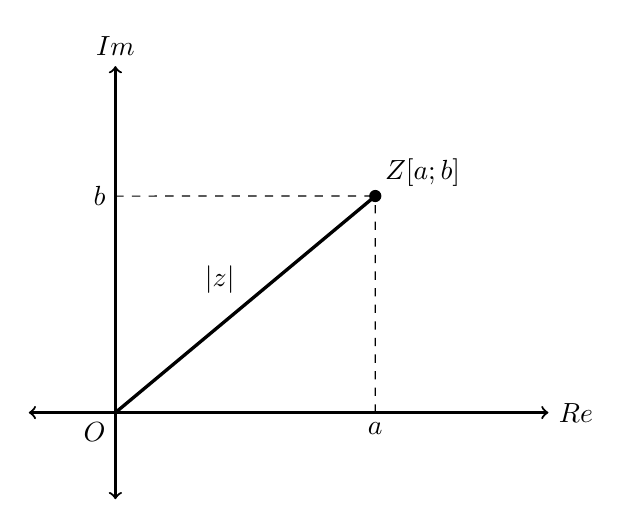
\begin{tikzpicture}[scale=1.1]
            \draw[<->, thick] (-1,0) -- (5,0) node[right] {$\operatorname{Re}$};
            \draw[<->, thick] (0,-1) -- (0,4) node[above] {$\operatorname{Im}$};
            \coordinate (O) at (0,0);
            \coordinate (Z) at (3,2.5);
            
            \draw[dashed] (3,0) -- (Z);
            \draw[dashed] (0,2.5) -- (Z);
            
            \draw[very thick] (O) -- (Z) node[midway, above left] {$|z|$};
            \node[below] at (3,0) {$a$};
            \node[left] at (0,2.5) {$b$};
            
            \fill (Z) circle (2pt) node[above right] {$Z[a;b]$};
            \node[below left] at (O) {$O$};
        \end{tikzpicture}
        \caption{Absolutní hodnota komplexního čísla jako vzdálenost od počátku}
    \end{center}
\end{figure}



\begin{examplebox}
    Určete absolutní hodnotu komplexního čísla
    \[
        z=3+4i.
    \]

    Reálná část komplexního čísla je
    \[
        a=3,
    \]

    zatímco jeho imaginární část je
    \[
        b=4.
    \]

    Dosadíme do vztahu pro absolutní hodnotu:
    \begin{align*}
        |z| &= \sqrt{3^2+4^2} \\
            &= \sqrt{9+16} \\
            &= \sqrt{25} \\
            &= 5.
    \end{align*}

    Komplexní číslo $z=3+4i$ je tedy v Gaussově rovině vzdáleno od počátku o $5$ jednotek.
\end{examplebox}

\begin{examplebox}
    Určete absolutní hodnotu komplexního čísla
    \[
        z=-\sqrt{3}+i.
    \]

    Dosadíme:
    \begin{align*}
        |z| &= \sqrt{(-\sqrt{3})^2+1^2} \\
            &= \sqrt{3+1} \\
            &= \sqrt{4} \\
            &= 2.
    \end{align*}

\end{examplebox}

Z definice absolutní hodnoty můžeme okamžitě odvodit několik základních vlastností. 
Protože druhé mocniny reálných čísel jsou vždy nezáporné, platí
\[
    |z|\geq0.
\]

Absolutní hodnota komplexního čísla je rovna nule právě tehdy, 
když jsou současně nulové jeho reálná i imaginární část, tedy
\[
    |z|=0 \Longleftrightarrow z=0.
\]

Komplexně sdružené číslo
\[
    \overline{z}=a-bi
\]

je v Gaussově rovině obrazem čísla $z=a+bi$ v osové souměrnosti podle reálné osy.
Oba body proto mají stejnou vzdálenost od počátku, a tedy
\[
    |\overline{z}|=|z|.
\]



\subsubsection*{Souvislost absolutní hodnoty a komplexně sdruženého čísla}
Při zavádění komplexně sdružených čísel jsme zjistili, že
\[
    z\overline{z} = (a+bi)(a-bi) = a^2+b^2.
\]

Z definice absolutní hodnoty zároveň platí
\[
    |z|^2 = \left(\sqrt{a^2+b^2}\right)^2 = a^2+b^2.
\]

Dostáváme proto velmi důležitý vztah
\[
    z\overline{z} = |z|^2.
\]

Odtud můžeme rovněž zapsat
\[
    |z| = \sqrt{z\overline{z}}.
\]

\begin{notebox}
    Pro každé komplexní číslo $z$ platí
    \[
        z\overline{z}=|z|^2.
    \]

    Tento vztah propojuje algebraický zápis komplexního čísla, 
    jeho komplexně sdružené číslo a jeho geometrickou vzdálenost od počátku Gaussovy roviny.

\end{notebox}


\subsubsection*{Vzdálenost dvou komplexních čísel}
Absolutní hodnota nám umožňuje určit nejen vzdálenost komplexního čísla od počátku,
ale také vzdálenost libovolných dvou komplexních čísel.
Mějme
\[
    z_1=a+bi
\]

a
\[
    z_2=c+di.
\]

Jejich rozdíl je
\[
    z_1-z_2 = (a-c)+(b-d)i.
\]

Absolutní hodnota tohoto rozdílu je
\[
    |z_1-z_2| = \sqrt{(a-c)^2+(b-d)^2},
\]

což je přesně známý vzorec pro vzdálenost dvou bodů
\[
    Z_1[a;b] \qquad\text{a}\qquad Z_2[c;d]
\]

v kartézské soustavě souřadnic.

\begin{definitionbox}
    Vzdálenost dvou komplexních čísel $z_1$ a $z_2$ v Gaussově rovině je
    \[
        d(z_1,z_2)=|z_1-z_2|.
    \]
\end{definitionbox}

\begin{examplebox}
    Určete vzdálenost komplexních čísel $z_1=4+3i$, $z_2=1-i$.

    Nejprve vypočítáme jejich rozdíl:
    \begin{align*}
        z_1-z_2 &= (4+3i)-(1-i) \\
                &= 4+3i-1+i \\
                &= 3+4i.
    \end{align*}

    Vzdálenost obou komplexních čísel je tedy
    \begin{align*}
        d(z_1,z_2)  &= |z_1-z_2| \\
                    &= |3+4i| \\
                    &= \sqrt{3^2+4^2} \\
                    &= 5.
    \end{align*}
\end{examplebox}


% ==================================================
% ===== GEOMETRICKÉ MNOŽINY KOMPLEXNÍCH ČÍSEL ======
% ==================================================

\subsection{Geometrické množiny komplexních čísel}

Absolutní hodnota komplexního čísla má v Gaussově rovině přirozený geometrický
význam. Pro komplexní číslo

\[
    z=a+bi
\]

představuje hodnota $|z|$ vzdálenost bodu $Z[a;b]$ od počátku soustavy souřadnic.
V předchozí části jsme tento pohled rozšířili také na vzdálenost dvou komplexních
čísel, přičemž pro libovolná komplexní čísla $z_1$ a $z_2$ platí

\[
    d(z_1,z_2)=|z_1-z_2|.
\]

Tento vztah nám umožňuje zapisovat pomocí komplexních čísel celé množiny bodů
v rovině. Rovnice nebo nerovnice obsahující absolutní hodnotu komplexního čísla
tak často není pouze algebraickou podmínkou, ale současně popisuje určitý
geometrický útvar v Gaussově rovině.


\subsubsection*{Kružnice}

Uvažujme pevně zvolené komplexní číslo

\[
    z_0=a+bi
\]

a proměnné komplexní číslo

\[
    z=x+yi.
\]

Rozdíl těchto čísel je

\[
    z-z_0=(x-a)+(y-b)i,
\]

a proto

\[
    |z-z_0|
    =
    \sqrt{(x-a)^2+(y-b)^2}.
\]

Výraz $|z-z_0|$ tedy představuje vzdálenost bodu $Z[x;y]$ od pevně zvoleného
bodu $Z_0[a;b]$.

Pokud požadujeme, aby tato vzdálenost byla stále rovna určitému kladnému číslu
$r$, dostáváme podmínku

\[
    |z-z_0|=r.
\]

Množinu všech bodů, které mají od pevného bodu stejnou vzdálenost $r$, však
známe již z geometrie. Jedná se o kružnici.

\begin{definitionbox}
    Nechť $z_0\in\mathbb{C}$ a $r>0$. Množina všech komplexních čísel $z$, pro která platí
    \[
        |z-z_0|=r,
    \]
    je \textbf{kružnice} se středem v bodě odpovídajícím komplexnímu číslu $z_0$ a poloměrem $r$.
\end{definitionbox}


\begin{examplebox}

    Znázorněte v Gaussově rovině množinu všech komplexních čísel $z$, pro která platí

    \[
        |z-3|=2.
    \]

    Výraz můžeme zapsat ve tvaru

    \[
        |z-(3+0i)|=2.
    \]

    Středem hledané kružnice je tedy bod

    \[
        S[3;0]
    \]

    a její poloměr je

    \[
        r=2.
    \]

    Pokud bychom chtěli podmínku převést do běžného souřadnicového zápisu, položíme

    \[
        z=x+yi.
    \]

    Potom

    \begin{align*}
        |z-3|
        &=
        |(x-3)+yi|\\
        &=
        \sqrt{(x-3)^2+y^2}.
    \end{align*}

    Rovnice

    \[
        |z-3|=2
    \]

    je tedy ekvivalentní rovnici

    \[
        (x-3)^2+y^2=4,
    \]

    což je skutečně rovnice kružnice se středem $S[3;0]$ a poloměrem $2$.

    \begin{center}
        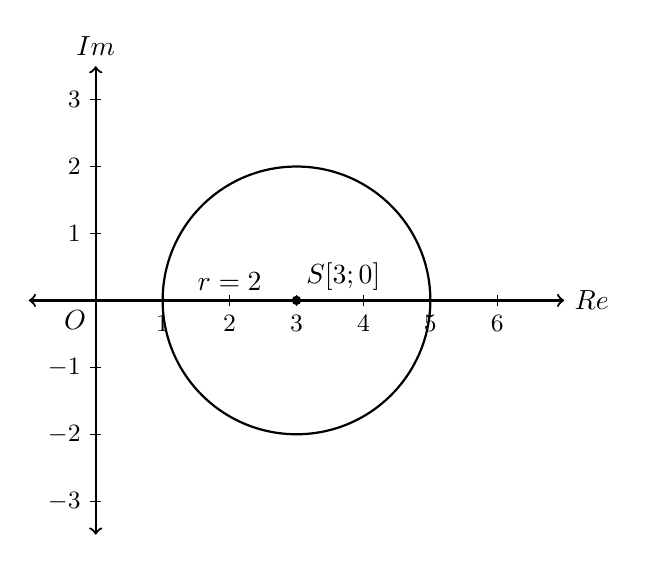
\begin{tikzpicture}[scale=0.85]
        
            \draw[<->, thick] (-1,0) -- (7,0)
                node[right] {$\operatorname{Re}$};
        
            \draw[<->, thick] (0,-3.5) -- (0,3.5)
                node[above] {$\operatorname{Im}$};
        
            \foreach \x in {1,2,3,4,5,6}
                \draw (\x,0.08) -- (\x,-0.08)
                    node[below] {\small $\x$};
        
            \foreach \y in {-3,-2,-1,1,2,3}
                \draw (0.08,\y) -- (-0.08,\y)
                    node[left] {\small $\y$};
        
            \draw[thick] (3,0) circle (2);
        
            \fill (3,0) circle (2pt)
                node[above right] {$S[3;0]$};
        
            \draw[dashed] (1,0) -- (3,0)
                node[midway, above] {$r=2$};
        
            \node[below left] at (0,0) {$O$};
        
        \end{tikzpicture}
    \end{center}

\end{examplebox}


\begin{notebox}
    Speciálním případem je rovnice
        \[
        |z|=r,
    \]

    kterou můžeme chápat jako
    \[
        |z-0|=r.
    \]
    Popisuje tedy kružnici se středem v počátku Gaussovy roviny a poloměrem $r$.
\end{notebox}


\subsubsection*{Kruh, vnitřek a vnějšek kružnice}
Rovnost
\[
    |z-z_0|=r
\]

vyjadřuje body, jejichž vzdálenost od bodu $z_0$ je právě $r$. Pokud však rovnost
nahradíme nerovností, získáme body, jejichž vzdálenost je menší nebo větší než
daný poloměr.

Pro $r>0$ tedy platí
\[
    |z-z_0|<r,
\]

jestliže bod leží uvnitř kružnice, avšak neleží na její hranici, zatímco podmínka
\[
    |z-z_0|\leq r
\]
popisuje celý kruh včetně jeho hraniční kružnice.

Naopak podmínka
\[
    |z-z_0|>r
\]
popisuje vnější oblast kružnice bez její hranice a podmínka
\[
    |z-z_0|\geq r
\]
zahrnuje kromě vnější oblasti také samotnou kružnici.

\begin{notebox}

    Pro $r>0$ můžeme geometrický význam jednotlivých podmínek shrnout následovně:

    \[
    \begin{array}{c|c}
        \text{Podmínka} & \text{Geometrický význam} \\ \hline
        |z-z_0|=r & \text{kružnice} \\
        |z-z_0|<r & \text{vnitřek kružnice bez hranice} \\
        |z-z_0|\leq r & \text{kruh včetně hranice} \\
        |z-z_0|>r & \text{vnější oblast bez kružnice} \\
        |z-z_0|\geq r & \text{vnější oblast včetně kružnice}
    \end{array}
    \]

\end{notebox}


\begin{examplebox}

    Znázorněte v Gaussově rovině množinu všech komplexních čísel $z$, pro která platí

    \[
        |z+3i|\leq4.
    \]

    Nejprve upravíme výraz uvnitř absolutní hodnoty do obvyklého tvaru:

    \[
        |z+3i|
        =
        |z-(-3i)|.
    \]

    Středem příslušného kruhu je tedy bod

    \[
        S[0;-3]
    \]

    a jeho poloměr je

    \[
        r=4.
    \]

    Protože se v zadání nachází znaménko $\leq$, hledáme celý kruh včetně jeho
    hraniční kružnice.

    \begin{center}
        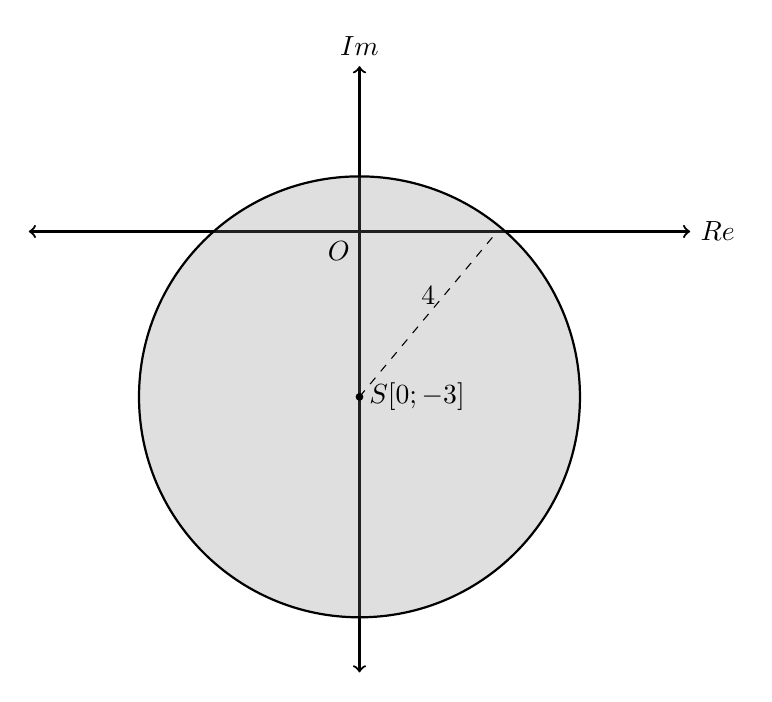
\begin{tikzpicture}[scale=0.7]
        
            \draw[<->, thick] (-6,0) -- (6,0)
                node[right] {$\operatorname{Re}$};
        
            \draw[<->, thick] (0,-8) -- (0,3)
                node[above] {$\operatorname{Im}$};
        
            \fill[gray, fill opacity=0.25] (0,-3) circle (4);
            \draw[thick] (0,-3) circle (4);
        
            \fill (0,-3) circle (2pt)
                node[right] {$S[0;-3]$};
        
            \draw[dashed] (0,-3) -- (2.5,0)
                node[midway, above] {$4$};
        
            \node[below left] at (0,0) {$O$};
        
        \end{tikzpicture}
    \end{center}

\end{examplebox}


\subsubsection*{Mezikruží}

Pomocí dvou nerovností můžeme popsat také oblast mezi dvěma soustřednými
kružnicemi. Například podmínka

\[
    2<|z-z_0|<5
\]

říká, že vzdálenost bodu $Z$ od bodu $Z_0$ je větší než $2$, ale současně menší
než $5$. Hledané body proto leží mezi kružnicemi s poloměry $2$ a $5$.

Obecně podmínka

\[
    r_1<|z-z_0|<r_2,
    \qquad
    0<r_1<r_2,
\]

popisuje \important{mezikruží} se středem v bodě $z_0$.

Podle použitých ostrých nebo neostrých nerovností mohou, ale nemusí jednotlivé
hraniční kružnice do výsledné množiny patřit.


\subsubsection*{Body stejně vzdálené od dvou komplexních čísel}

Uvažujme nyní dvě různá pevná komplexní čísla $z_1$ a $z_2$. Podmínka

\[
    |z-z_1|=|z-z_2|
\]

říká, že hledaný bod $Z$ má od bodů $Z_1$ a $Z_2$ stejnou vzdálenost.

Z geometrie víme, že množinou všech bodů stejně vzdálených od dvou různých bodů
je osa úsečky, která tyto body spojuje.

\begin{definitionbox}

Jsou-li $z_1,z_2\in\mathbb{C}$ dvě různá komplexní čísla, potom rovnice

\[
    |z-z_1|=|z-z_2|
\]

popisuje v Gaussově rovině \textbf{osu úsečky} $Z_1Z_2$.

\end{definitionbox}


\begin{examplebox}

Znázorněte množinu všech komplexních čísel $z$, pro která platí

\[
    |z-(1+i)|=|z-(3-i)|.
\]

Komplexním číslům

\[
    z_1=1+i
    \qquad\text{a}\qquad
    z_2=3-i
\]

odpovídají body

\[
    Z_1[1;1]
    \qquad\text{a}\qquad
    Z_2[3;-1].
\]

Hledáme všechny body, které jsou od bodů $Z_1$ a $Z_2$ stejně vzdálené, takže
výsledkem bude osa úsečky $Z_1Z_2$.

Výsledek můžeme ověřit také algebraicky. Položíme

\[
    z=x+yi.
\]

Potom

\[
    |z-(1+i)|=|z-(3-i)|
\]

vede na

\[
    \sqrt{(x-1)^2+(y-1)^2}
    =
    \sqrt{(x-3)^2+(y+1)^2}.
\]

Po umocnění obou stran dostáváme

\[
    (x-1)^2+(y-1)^2
    =
    (x-3)^2+(y+1)^2.
\]

Po úpravě

\[
    x-y-2=0,
\]

tedy

\[
    y=x-2.
\]

Hledaná množina je proto přímka

\[
    y=x-2.
\]

\begin{center}
\begin{tikzpicture}[scale=0.9]

    \draw[<->, thick] (-1,0) -- (6,0)
        node[right] {$\operatorname{Re}$};

    \draw[<->, thick] (0,-4) -- (0,4)
        node[above] {$\operatorname{Im}$};

    \fill (1,1) circle (2pt)
        node[above left] {$Z_1$};

    \fill (3,-1) circle (2pt)
        node[below right] {$Z_2$};

    \draw[dashed] (1,1) -- (3,-1);

    \draw[thick] (-1,-3) -- (6,4)
        node[above right] {$y=x-2$};

    \node[below left] at (0,0) {$O$};

\end{tikzpicture}
\end{center}

\end{examplebox}


\subsubsection*{Poloroviny určené vzdáleností}

Pokud rovnost vzdáleností nahradíme nerovností, získáme jednu z polorovin
určených osou úsečky $Z_1Z_2$.

Podmínka

\[
    |z-z_1|<|z-z_2|
\]

vyjadřuje všechny body, které jsou blíže k bodu $Z_1$ než k bodu $Z_2$, zatímco

\[
    |z-z_1|>|z-z_2|
\]

popisuje body bližší k bodu $Z_2$.

Při použití znamének $\leq$ nebo $\geq$ patří do výsledné množiny také hraniční
přímka.

\begin{examplebox}

Znázorněte v Gaussově rovině množinu všech komplexních čísel $z$, pro která platí

\[
    |z+1|\leq|z-i|.
\]

Číslo $-1$ odpovídá bodu

\[
    A[-1;0],
\]

zatímco číslo $i$ odpovídá bodu

\[
    B[0;1].
\]

Podmínka tedy požaduje všechny body, jejichž vzdálenost od bodu $A$ je menší
nebo rovna jejich vzdálenosti od bodu $B$.

Položíme

\[
    z=x+yi.
\]

Potom

\[
    \sqrt{(x+1)^2+y^2}
    \leq
    \sqrt{x^2+(y-1)^2}.
\]

Po umocnění obou stran dostáváme

\[
    (x+1)^2+y^2
    \leq
    x^2+(y-1)^2.
\]

Po úpravě

\[
    x+y\leq0.
\]

Hledanou množinou je tedy polorovina

\[
    y\leq-x,
\]

včetně její hraniční přímky

\[
    y=-x.
\]

\end{examplebox}


\begin{notebox}

U nerovností tvaru

\[
    |z-z_1|\leq|z-z_2|
\]

často není nutné provádět celý algebraický výpočet. Stačí si uvědomit, že
hranicí je osa úsečky $Z_1Z_2$ a poté určit, na které straně této přímky leží
bod $Z_1$. Právě tato polorovina je množinou bodů, které jsou k $Z_1$ alespoň
tak blízko jako k $Z_2$.

\end{notebox}


\subsubsection*{Přímky určené reálnou a imaginární částí}

Některé množiny komplexních čísel můžeme popsat také přímo pomocí jejich reálné
nebo imaginární části.

Je-li

\[
    z=x+yi,
\]

potom podmínka

\[
    \operatorname{Re}(z)=a
\]

znamená

\[
    x=a,
\]

a popisuje tedy přímku rovnoběžnou s imaginární osou.

Podobně podmínka

\[
    \operatorname{Im}(z)=b
\]

znamená

\[
    y=b,
\]

a popisuje přímku rovnoběžnou s reálnou osou.

Protože pro komplexní číslo $z=x+yi$ platí

\[
    z+\overline{z}=2x
\]

a

\[
    z-\overline{z}=2yi,
\]

můžeme stejným způsobem geometricky interpretovat také rovnice obsahující
komplexně sdružené číslo.


\begin{examplebox}

Znázorněte v Gaussově rovině množinu všech komplexních čísel $z$, pro která platí

\[
    z+\overline{z}=-2.
\]

Položíme

\[
    z=x+yi,
    \qquad
    \overline{z}=x-yi.
\]

Potom

\begin{align*}
    z+\overline{z}
    &=
    x+yi+x-yi\\
    &=
    2x.
\end{align*}

Rovnice tedy přejde na

\[
    2x=-2,
\]

odkud

\[
    x=-1.
\]

Hledanou množinou je tedy přímka

\[
    \operatorname{Re}(z)=-1,
\]

která je rovnoběžná s imaginární osou.

\end{examplebox}


\begin{examplebox}

Znázorněte v Gaussově rovině množinu všech komplexních čísel $z$, pro která platí

\[
    z-\overline{z}=4i.
\]

Pro $z=x+yi$ platí

\[
    z-\overline{z}=2yi.
\]

Dostáváme proto

\[
    2yi=4i,
\]

tedy

\[
    y=2.
\]

Výsledkem je přímka

\[
    \operatorname{Im}(z)=2,
\]

která je rovnoběžná s reálnou osou.

\end{examplebox}


\begin{notebox}

Při geometrickém znázorňování množin komplexních čísel je vhodné nejprve zjistit,
jaký geometrický význam má použitý výraz. Především platí

\[
    |z-z_0|
\]

jako vzdálenost bodu $Z$ od pevného bodu $Z_0$, zatímco

\[
    |z-z_1|=|z-z_2|
\]

vyjadřuje stejnou vzdálenost od dvou bodů.

Díky tomuto pohledu lze mnoho zdánlivě komplikovaných rovnic a nerovnic vyřešit
geometricky bez rozsáhlých algebraických úprav.

\end{notebox}


% ==================================================
% =================== ARGUMENT ======================
% ==================================================

\subsection{Argument komplexního čísla}

Absolutní hodnota nám říká, jak daleko se bod představující komplexní číslo
nachází od počátku Gaussovy roviny, ale sama o sobě jeho polohu neurčuje.
Například všechna komplexní čísla ležící na kružnici se středem v počátku
a poloměrem $2$ mají stejnou absolutní hodnotu
\[
    |z|=2,
\]

přestože se mohou nacházet na různých místech této kružnice.

Abychom mohli polohu komplexního čísla popsat úplněji, potřebujeme kromě jeho
vzdálenosti od počátku znát také směr, ve kterém se bod nachází. 
Tento směr určíme pomocí orientovaného úhlu mezi kladnou částí reálné osy a
polopřímkou vedoucí z počátku $O$ přes bod $Z$. 
Kladný směr měření úhlu volíme proti směru hodinových ručiček.

\begin{definitionbox}
    Nechť $z\neq0$ je komplexní číslo, kterému v Gaussově rovině odpovídá bod $Z$.
    \textbf{Argumentem komplexního čísla} $z$ nazýváme každý orientovaný úhel
    $\varphi$, který svírá kladná část reálné osy s polopřímkou $OZ$.
\end{definitionbox}

\begin{figure}[ht]
    \begin{center}
        \begin{tikzpicture}[scale=1.15]
            \draw[<->, thick] (-1,0) -- (5,0)
                node[right] {$\operatorname{Re}$};
            \draw[<->, thick] (0,-1) -- (0,4)
                node[above] {$\operatorname{Im}$};
            \coordinate (O) at (0,0);
            \coordinate (Z) at (3.5,2.5);
            \draw[very thick] (O) -- (Z)
                node[midway, above left] {$|z|$};
            \fill (Z) circle (2pt)
                node[above right] {$Z$};
            \draw[->, thick]
                (1,0)
                arc[start angle=0,end angle=35.5,radius=1];
            \node at (1.25,0.45) {$\varphi$};
            \node[below left] at (O) {$O$};
        \end{tikzpicture}
        \caption{Argument komplexního čísla}
    \end{center}
\end{figure}

Argument komplexního čísla není určen jediným reálným číslem. 
Pokud totiž úhel zvětšíme nebo zmenšíme o celý oběh
\[
    2\pi,
\]

dostaneme opět stejnou polopřímku a tedy stejnou polohu bodu $Z$. 
Je-li proto $\varphi$ jedním argumentem komplexního čísla, pak jsou jeho argumenty také
\[
    \varphi+2\pi, \qquad \varphi-2\pi, \qquad \varphi+4\pi
\]

a obecně všechny úhly
\[
    \varphi+2k\pi, \qquad k\in\mathbb{Z}.
\]

\begin{notebox}
    Argument čísla $z=0$ není definován, protože nulové komplexní číslo odpovídá
    počátku Gaussovy roviny a z počátku k němu nelze určit žádný jednoznačný směr.
\end{notebox}

Abychom nemuseli při každém výpočtu pracovat s nekonečně mnoha úhly, vybereme
z nich jeden jako \important{hlavní argument}.
V této učebnici budeme hlavní argument označovat symbolem
\[
    \operatorname{Arg} z
\]

a volit jej z intervalu
\[
    \operatorname{Arg} z\in\langle0;2\pi).
\]

Všechny argumenty daného komplexního čísla potom získáme přičtením celočíselného
násobku $2\pi$ k jeho hlavnímu argumentu:
\[
    \varphi=\operatorname{Arg}z+2k\pi, \qquad k\in\mathbb{Z}.
\]


\subsubsection*{Určení argumentu z algebraického tvaru}
Uvažujme komplexní číslo
\[
    z=a+bi, \qquad z\neq0,
\]

jehož absolutní hodnota je
\[
    |z|=\sqrt{a^2+b^2}.
\]

Bod $Z[a;b]$, jeho kolmý průmět na reálnou osu a počátek $O$ vytvářejí pravoúhlý trojúhelník. 
Z definic goniometrických funkcí proto získáváme vztahy
\[
    \cos\varphi=\frac{a}{|z|}
\]

a
\[
    \sin\varphi=\frac{b}{|z|}.
\]

Odtud můžeme naopak vyjádřit reálnou a imaginární část ve tvaru
\[
    a=|z|\cos\varphi
\]

a
\[
    b=|z|\sin\varphi.
\]

Při určování argumentu je zároveň nutné sledovat, ve které části Gaussovy roviny bod $Z$ leží.
Znaménka reálné a imaginární části nám okamžitě určují příslušný kvadrant:

\[
    \begin{array}{c|c|c}
        \text{Kvadrant} & \operatorname{Re}(z) & \operatorname{Im}(z) \\ \hline
        \mathrm{I.}   & + & + \\
        \mathrm{II.}  & - & + \\
        \mathrm{III.} & - & - \\
        \mathrm{IV.}  & + & -
    \end{array}
\]

\begin{notebox}
    Při určování argumentu nestačí bez dalšího uvažování použít pouze vztah
    \[
        \tan\varphi=\frac{b}{a},
    \]
    protože tangens má stejnou hodnotu pro úhly lišící se o $\pi$. 
    Je proto vždy nutné zohlednit také znaménka reálné a imaginární části a určit, 
    ve kterém kvadrantu se bod $Z$ nachází.
\end{notebox}


\begin{examplebox}
    Určete absolutní hodnotu a hlavní argument komplexního čísla $z=1+\sqrt{3}i$.

    Nejprve určíme absolutní hodnotu:
    \begin{align*}
        |z| &= \sqrt{1^2+(\sqrt{3})^2}\\
            &= \sqrt{1+3}\\
            &= 2.
    \end{align*}

    Pro argument tedy platí
    \[
        \cos\varphi=\frac{1}{2}, \qquad \sin\varphi=\frac{\sqrt{3}}{2}.
    \]

    Obě hodnoty jsou kladné, takže bod $Z$ leží v prvním kvadrantu. Dostáváme proto
    \[
        \operatorname{Arg}z=\frac{\pi}{3}.
    \]

    Všechny argumenty tohoto komplexního čísla mají tvar
    \[
        \varphi=\frac{\pi}{3}+2k\pi, \qquad k\in\mathbb{Z}.
    \]
\end{examplebox}


\begin{examplebox}
    Určete absolutní hodnotu a hlavní argument komplexního čísla
    \[
        z=-1+\sqrt{3}i.
    \]

    Absolutní hodnota je
    \[
        |z| = \sqrt{(-1)^2+(\sqrt{3})^2} = 2.
    \]

    Dále platí
    \[
        \cos\varphi=-\frac{1}{2}, \qquad \sin\varphi=\frac{\sqrt{3}}{2}.
    \]

    Reálná část je záporná a imaginární část kladná, takže bod leží ve druhém kvadrantu. 
    Hlavní argument je proto
    \[
        \operatorname{Arg}z=\frac{2\pi}{3}.
    \]

    Všechny argumenty mají tvar
    \[
        \varphi=\frac{2\pi}{3}+2k\pi, \qquad k\in\mathbb{Z}.
    \]
\end{examplebox}


Komplexní číslo $z\neq0$ jsme tedy nyní schopni popsat dvěma různými způsoby.
V algebraickém tvaru jej určujeme pomocí jeho reálné a imaginární části
\[
    z=a+bi,
\]

zatímco geometricky jej můžeme určit pomocí jeho absolutní hodnoty $|z|$ a argumentu $\varphi$.

Právě spojení těchto dvou údajů nás přivede k dalšímu důležitému způsobu zápisu
komplexního čísla, který nazýváme \important{goniometrickým tvarem komplexního čísla}.



% ==================================================
% ============ GONIOMETRICKÝ TVAR ==================
% ==================================================

\section{Goniometrický tvar komplexního čísla}
V předchozí části jsme ukázali, že nenulové komplexní číslo
\[
    z=a+bi
\]
můžeme v Gaussově rovině popsat pomocí jeho absolutní hodnoty
\[
    |z|=\sqrt{a^2+b^2}
\]
a argumentu $\varphi$. 
Z pravoúhlého trojúhelníku, který vznikne spuštěním kolmice z bodu $Z[a;b]$ na reálnou osu, 
jsme získali vztahy
\[
    \cos\varphi=\frac{a}{|z|}
\]

a
\[
    \sin\varphi=\frac{b}{|z|}.
\]

Odtud můžeme vyjádřit reálnou a imaginární část komplexního čísla jako
\[
    a=|z|\cos\varphi
\]

a
\[
    b=|z|\sin\varphi.
\]

Tyto vztahy nyní dosadíme do algebraického tvaru komplexního čísla
\[
    z=a+bi.
\]

Dostáváme
\begin{align*}
    z   &= |z|\cos\varphi+i|z|\sin\varphi \\
        &= |z|\left(\cos\varphi+i\sin\varphi\right).
\end{align*}

Tím jsme získali nový způsob zápisu komplexního čísla, který nazýváme
\important{goniometrickým tvarem komplexního čísla}.

\begin{definitionbox}
    Nechť $z\neq0$ je komplexní číslo, $|z|$ jeho absolutní hodnota a $\varphi$
    jeden z jeho argumentů. Potom zápis
    \[
        z=|z|\left(\cos\varphi+i\sin\varphi\right)
    \]
    nazýváme \textbf{goniometrickým tvarem komplexního čísla}.
    
    Často označujeme
    \[
        r=|z|,
    \]

    a goniometrický tvar potom zapisujeme také jako
    \[
        z=r\left(\cos\varphi+i\sin\varphi\right),
        \qquad r>0.
    \]
\end{definitionbox}

V goniometrickém tvaru tedy komplexní číslo nepopisujeme přímo pomocí jeho reálné
a imaginární části, ale pomocí dvou geometrických údajů. Číslo
\[
    r=|z|
\]

udává vzdálenost odpovídajícího bodu od počátku Gaussovy roviny, 
zatímco úhel $\varphi$ určuje jeho polohu vzhledem ke kladné části reálné osy.


\begin{figure}[ht]
    \begin{center}
        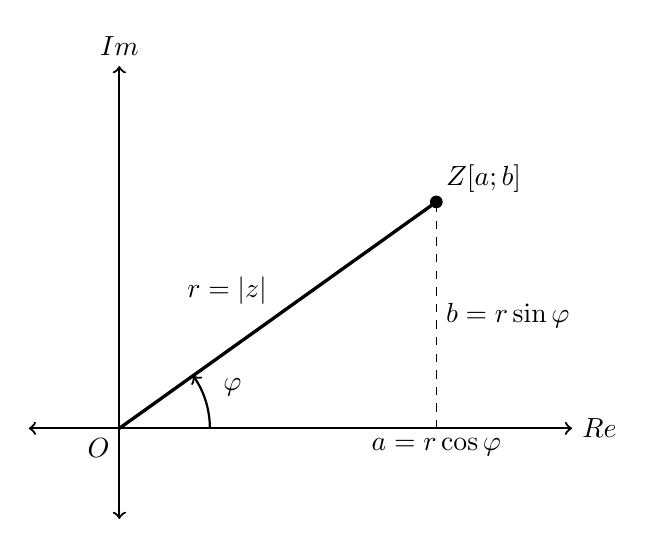
\begin{tikzpicture}[scale=1.15]

            \draw[<->, thick] (-1,0) -- (5,0)
                node[right] {$\operatorname{Re}$};

            \draw[<->, thick] (0,-1) -- (0,4)
                node[above] {$\operatorname{Im}$};

            \coordinate (O) at (0,0);
            \coordinate (Z) at (3.5,2.5);
            \coordinate (A) at (3.5,0);

            \draw[very thick] (O) -- (Z)
                node[midway, above left] {$r=|z|$};

            \draw[dashed] (A) -- (Z);

            \fill (Z) circle (2pt)
                node[above right] {$Z[a;b]$};

            \node[below] at (A) {$a=r\cos\varphi$};
            \node[right] at (3.5,1.25) {$b=r\sin\varphi$};

            \draw[->, thick]
                (1,0)
                arc[start angle=0,end angle=35.5,radius=1];

            \node at (1.25,0.45) {$\varphi$};
            \node[below left] at (O) {$O$};

        \end{tikzpicture}

        \caption{Geometrický význam goniometrického tvaru komplexního čísla}
    \end{center}
\end{figure}


\begin{notebox}
    Goniometrický tvar komplexního čísla není jednoznačný vzhledem k argumentu.
    Jestliže je $\varphi$ argumentem komplexního čísla, 
    potom stejnému bodu odpovídají také úhly
    \[
        \varphi+2k \pi , \qquad k \in \mathbb{Z}.
    \]

    Proto můžeme stejné komplexní číslo zapsat ve tvaru
    \[
        z = |z| \left( \cos(\varphi+2k\pi) + i\sin(\varphi+2k\pi) \right),
        \qquad k \in \mathbb{Z}.
    \]

    Chceme-li jeden základní zápis, používáme hlavní argument $\operatorname{Arg}z$.
\end{notebox}


\subsection{Převod z algebraického do goniometrického tvaru}
Při převodu komplexního čísla z algebraického tvaru
\[
    z=a+bi
\]
do tvaru goniometrického potřebujeme určit dvě hodnoty. 
Nejprve vypočítáme absolutní hodnotu
\[
    |z|=\sqrt{a^2+b^2}
\]

a následně určíme argument $\varphi$, 
přičemž musíme zohlednit také polohu bodu $Z[a;b]$ v Gaussově rovině.

Poté pouze dosadíme do vztahu
\[
    z=|z|\left(\cos\varphi+i\sin\varphi\right).
\]


\begin{examplebox}
    Zapište komplexní číslo $z=1+\sqrt{3}i$ v goniometrickém tvaru.

    Nejprve určíme jeho absolutní hodnotu:
    \begin{align*}
        |z| &= \sqrt{1^2+(\sqrt{3})^2} \\
            &= \sqrt{1+3} \\
            &= 2.
    \end{align*}

    Pro argument platí
    \[
        \cos\varphi=\frac{1}{2}, \qquad \sin\varphi=\frac{\sqrt{3}}{2}.
    \]

    Bod odpovídající komplexnímu číslu leží v prvním kvadrantu, a proto

    \[
        \operatorname{Arg}z=\frac{\pi}{3}.
    \]

    Goniometrický tvar je tedy

    \[
        z= 2\left( \cos\frac{\pi}{3} + i\sin\frac{\pi}{3}\right).
    \]
\end{examplebox}

\begin{examplebox}
    Zapište komplexní číslo $z=-1+\sqrt{3}i$ v goniometrickém tvaru.

    Absolutní hodnota je
    \[
        |z| = \sqrt{(-1)^2+(\sqrt{3})^2} = 2.
    \]

    Dále platí
    \[
        \cos\varphi=-\frac{1}{2}, \qquad \sin\varphi=\frac{\sqrt{3}}{2}.
    \]

    Bod leží ve druhém kvadrantu, takže
    \[
        \operatorname{Arg}z=\frac{2\pi}{3}.
    \]

    Goniometrický tvar čísla je proto
    \[
        z= 2\left(\cos\frac{2\pi}{3} + i\sin\frac{2\pi}{3}\right).
    \]
\end{examplebox}


\begin{examplebox}
    Zapište komplexní číslo $z=-2-2i$ v goniometrickém tvaru.

    Nejprve určíme absolutní hodnotu:
    \begin{align*}
        |z| &= \sqrt{(-2)^2+(-2)^2} \\
            &= \sqrt{4+4} \\
            &= \sqrt{8} \\
            &= 2\sqrt{2}.
    \end{align*}

    Protože reálná i imaginární část jsou záporné, bod leží ve třetím kvadrantu.
    Pro argument platí

    \[
        \cos\varphi = -\frac{2}{2\sqrt{2}} = -\frac{\sqrt{2}}{2}
    \]
    a
    \[
        \sin\varphi = -\frac{2}{2\sqrt{2}} = -\frac{\sqrt{2}}{2}.
    \]

    Hlavní argument je tedy
    \[
        \operatorname{Arg}z=\frac{5\pi}{4}.
    \]

    Goniometrický tvar je
    \[
        z = 2\sqrt{2} \left(\cos\frac{5\pi}{4} + i\sin\frac{5\pi}{4}\right).
    \]
\end{examplebox}


\begin{notebox}
    U čísel ležících přímo na reálné nebo imaginární ose lze argument určit
    přímo z jejich polohy v Gaussově rovině:

    \[
        \begin{array}{c|c}
            \text{Poloha komplexního čísla} & \operatorname{Arg}z \\ \hline
            z>0 & 0 \\
            z=bi,\ b>0 & \frac{\pi}{2} \\
            z<0 & \pi \\
            z=bi,\ b<0 & \frac{3\pi}{2}
        \end{array}
    \]

    Pro $z=0$ argument definován není.
\end{notebox}


\begin{examplebox}
    Zapište komplexní číslo $z=-3i$ v goniometrickém tvaru.

    Jeho absolutní hodnota je
    \[
        |z|=3.
    \]

    Bod leží na záporné části imaginární osy, a proto
    \[
        \operatorname{Arg}z=\frac{3\pi}{2}.
    \]

    Dostáváme tedy
    \[
        z = 3\left(\cos\frac{3\pi}{2} + i\sin\frac{3\pi}{2}\right).
    \]
\end{examplebox}


\subsection{Převod z goniometrického do algebraického tvaru}
Převod opačným směrem je zpravidla jednodušší. 
Máme-li komplexní číslo v goniometrickém tvaru
\[
    z=r\left(\cos\varphi+i\sin\varphi\right),
\]

stačí určit hodnoty goniometrických funkcí a roznásobit závorku:
\[
    z = r\cos\varphi + ri\sin\varphi.
\]

Odtud přímo získáváme
\[
    \operatorname{Re}(z)=r\cos\varphi
\]

a
\[
    \operatorname{Im}(z)=r\sin\varphi.
\]


\begin{examplebox}
    Zapište komplexní číslo $z = 4\left(\cos\frac{2\pi}{3} + i\sin\frac{2\pi}{3}\right)$ v algebraickém tvaru.

    Známe hodnoty
    \[
        \cos\frac{2\pi}{3}=-\frac{1}{2}
    \]
    a
    \[
        \sin\frac{2\pi}{3}=\frac{\sqrt{3}}{2}.
    \]

    Dosadíme:

    \begin{align*}
        z   &= 4\left(-\frac{1}{2} + i\frac{\sqrt{3}}{2}\right) \\
            &= -2+2\sqrt{3}i.
    \end{align*}

    Algebraický tvar je tedy
    \[
        z=-2+2\sqrt{3}i.
    \]
\end{examplebox}


\begin{examplebox}
    Zapište komplexní číslo $z = 6\left(\cos\frac{7\pi}{6} + i\sin\frac{7\pi}{6}\right)$ v algebraickém tvaru.

    Platí
    \[
        \cos\frac{7\pi}{6} = -\frac{\sqrt{3}}{2}
    \]

    a
    \[
        \sin\frac{7\pi}{6} = -\frac{1}{2}.
    \]

    Proto
    \begin{align*}
        z   &= 6\left(-\frac{\sqrt{3}}{2} - \frac{1}{2}i\right)\\
            &= -3\sqrt{3}-3i.
    \end{align*}
\end{examplebox}


\begin{notebox}
    Algebraický a goniometrický tvar popisují stejné komplexní číslo, 
    pouze používají jiné údaje.

    V algebraickém tvaru
    \[
        z=a+bi
    \]

    pracujeme s reálnou a imaginární částí, zatímco v goniometrickém tvaru
    \[
        z=r\left(\cos\varphi+i\sin\varphi\right)
    \]

    pracujeme s absolutní hodnotou
    \[
        r=|z|
    \]
    a argumentem $\varphi$.

    Mezi oběma způsoby zápisu platí vztahy
    \[
        a=r\cos\varphi, \qquad b=r\sin\varphi.
    \]
\end{notebox}

% ==================================================
% ===== OPERACE V GONIOMETRICKÉM TVARU =============
% ==================================================

\section{Operace s komplexními čísly v goniometrickém tvaru}
Goniometrický tvar komplexního čísla není výhodnější pro všechny početní operace.
Například při sčítání nebo odčítání komplexních čísel je zpravidla jednodušší
pracovat s algebraickým tvarem
\[
    z=a+bi,
\]

protože můžeme přímo sčítat nebo odčítat reálné a imaginární části.

Výhoda goniometrického tvaru se však výrazně projeví při
\important{násobení}, \important{dělení} a později také při
\important{umocňování} komplexních čísel.


% --------------------------------------------------
% NÁSOBENÍ
% --------------------------------------------------

\subsection{Násobení komplexních čísel v goniometrickém tvaru}

Uvažujme dvě nenulová komplexní čísla

\[
    z_1 = r_1 \left(\cos\varphi_1 + i\sin\varphi_1\right)
\]

a
\[
    z_2 = r_2 \left(\cos\varphi_2 + i\sin\varphi_2\right),
\]

kde
\[
    r_1=|z_1|, \qquad r_2=|z_2|.
\]

Jejich součin je
\begin{align*}
    z_1z_2  &= r_1 \cdot r_2 \left(\cos\varphi_1+i\sin\varphi_1\right) \cdot \left(\cos\varphi_2+i\sin\varphi_2\right).
\end{align*}

Roznásobíme závorky a dostáváme:

\begin{align*}
    z_1z_2  &= r_1 \cdot r_2 \Bigl( \cos\varphi_1\cos\varphi_2 + i\cos\varphi_1\sin\varphi_2 + i\sin\varphi_1\cos\varphi_2 + i^2\sin\varphi_1\sin\varphi_2 \Bigr).
\end{align*}

Protože
\[
    i^2=-1,
\]

upravíme a dostáváme

\begin{align*}
    z_1z_2  &= r_1 \cdot r_2 \Bigl( \cos\varphi_1\cos\varphi_2 - \sin\varphi_1\sin\varphi_2 + i(\sin\varphi_1\cos\varphi_2 + \cos\varphi_1\sin\varphi_2)\Bigr).
\end{align*}

Nyní využijeme známé součtové vzorce
\[
    \cos(\alpha+\beta) = \cos\alpha\cos\beta - \sin\alpha\sin\beta
\]

a
\[
    \sin(\alpha+\beta) = \sin\alpha\cos\beta + \cos\alpha\sin\beta.
\]

Výraz se proto zjednoduší na

\[
    z_1z_2 = r_1r_2 \left(
                        \cos(\varphi_1+\varphi_2)
                        +
                        i\sin(\varphi_1+\varphi_2)
                    \right).
\]

\begin{notebox}
    Při násobení komplexních čísel v goniometrickém tvaru
    \textbf{násobíme jejich absolutní hodnoty a sčítáme jejich argumenty}.

    Pro
    \[
        z_1 = r_1 \left(\cos\varphi_1+i\sin\varphi_1\right)
    \]

    a
    \[
        z_2 = r_2 \left(\cos\varphi_2+i\sin\varphi_2\right)
    \]

    platí
    \[
        z_1z_2 = r_1r_2 \left(
                            \cos(\varphi_1+\varphi_2)
                            +
                            i\sin(\varphi_1+\varphi_2)
                        \right).
    \]

    Současně tedy platí
    \[
        |z_1z_2| = |z_1|\cdot|z_2|.
    \]
\end{notebox}

Z geometrického hlediska má tento vztah jednoduchý význam. 
Při násobení dvou komplexních čísel se jejich vzdálenosti od počátku násobí 
a jejich úhly vůči kladné části reálné osy se sčítají.

\begin{examplebox}
    Vypočítejte součin komplexních čísel
    \[
        z_1 = 2 \left(
                    \cos\frac{\pi}{6}
                    +
                    i\sin\frac{\pi}{6}
                \right)
    \]
    a
    \[
        z_2 = 3 \left(
                    \cos\frac{\pi}{4}
                    +
                    i\sin\frac{\pi}{4}
                \right).
    \]

    Absolutní hodnoty vynásobíme:
    \[
        |z_1z_2| = 2 \cdot 3 = 6.
    \]

    Argumenty sečteme:

    \begin{align*}
        \varphi &= \frac{\pi}{6} + \frac{\pi}{4}\\
                &= \frac{2\pi}{12} + \frac{3\pi}{12}\\
                &= \frac{5\pi}{12}.
    \end{align*}

    Dostáváme tedy
    \[
        z_1z_2 = 6  \left(
                        \cos\frac{5\pi}{12}
                        +
                        i\sin\frac{5\pi}{12}
                    \right).
    \]          
\end{examplebox}


\begin{examplebox}
    Vypočítejte součin
    \[
        z_1 = 2 \left(
                    \cos\frac{3\pi}{4}
                    +
                    i\sin\frac{3\pi}{4}
                \right)
    \]
    a
    \[    
        z_2 = 4 \left(
                    \cos\frac{5\pi}{6}
                    +
                    i\sin\frac{5\pi}{6}
                \right).
    \]

    Absolutní hodnota součinu je
    \[
        |z_1z_2| = 2 \cdot 4 = 8.
    \]

    Argument součinu je

    \begin{align*}
        \varphi &= \frac{3\pi}{4} + \frac{5\pi}{6}\\
                &= \frac{9\pi}{12} + \frac{10\pi}{12}\\
                &= \frac{19\pi}{12}.
    \end{align*}

    Proto
    \[
        z_1z_2 = 8  \left(
                        \cos\frac{19\pi}{12}
                        +
                        i\sin\frac{19\pi}{12}
                    \right).
    \]

    Protože
    \[
        \frac{19\pi}{12}\in\langle0;2\pi),
    \]
    jde zároveň o hlavní argument výsledného komplexního čísla.
\end{examplebox}


% --------------------------------------------------
% DĚLENÍ
% --------------------------------------------------
\subsection{Dělení komplexních čísel v goniometrickém tvaru}
Podobně jako násobení můžeme v goniometrickém tvaru jednoduše provádět 
také dělení komplexních čísel.

Uvažujme
\[
    z_1 = r_1   \left(
                    \cos\varphi_1+i\sin\varphi_1
                \right)
\]          

a
\[
    z_2 = r_2   \left(
                    \cos\varphi_2+i\sin\varphi_2
                \right),
    \qquad z_2\neq0.
\]

Pro jejich podíl platí

\[
    \frac{z_1}{z_2} = \frac{r_1}{r_2}   \left(
                                            \cos(\varphi_1-\varphi_2)
                                            +
                                            i\sin(\varphi_1-\varphi_2)
                                        \right).
\]

\begin{notebox}
    Při dělení komplexních čísel v goniometrickém tvaru
    \textbf{dělíme jejich absolutní hodnoty a odečítáme jejich argumenty}.

    Platí tedy
    \[
        \frac{z_1}{z_2} = \frac{r_1}{r_2}   \left(
                                                \cos(\varphi_1-\varphi_2)
                                                +
                                                i\sin(\varphi_1-\varphi_2)
                                            \right),
        \qquad z_2\neq0.
    \]

    Současně platí
    \[
        \left| \frac{z_1}{z_2} \right| = \frac{|z_1|}{|z_2|}.
    \]
\end{notebox}


\begin{examplebox}
    Vypočítejte podíl komplexních čísel
    \[
        z_1 = 8 \left(
                    \cos\frac{5\pi}{6}
                    +
                    i\sin\frac{5\pi}{6}
                \right)
    \]
    a
    \[
        z_2 = 2 \left(
                    \cos\frac{\pi}{3}
                    +
                    i\sin\frac{\pi}{3}
                \right).
    \]

    Absolutní hodnoty vydělíme:
    \[
        \frac{|z_1|}{|z_2|} = \frac{8}{2} = 4.
    \]

    Argumenty odečteme:
    \begin{align*}
        \varphi &= \frac{5\pi}{6} - \frac{\pi}{3} \\
                &= \frac{5\pi}{6} - \frac{2\pi}{6} \\
                &= \frac{\pi}{2}.
    \end{align*}

    Výsledkem je
    \[
        \frac{z_1}{z_2} = 4 \left(
                                \cos\frac{\pi}{2}
                                +
                                i\sin\frac{\pi}{2}
                            \right).
    \]

    Protože
    \[
        \cos\frac{\pi}{2}=0 \qquad\text{a}\qquad \sin\frac{\pi}{2}=1,
    \]

    můžeme výsledek zapsat také v algebraickém tvaru
    \[
        \frac{z_1}{z_2}=4i.
    \]
\end{examplebox}


\begin{examplebox}
    Vypočítejte podíl
    \[
        z_1 = 6 \left(
                    \cos\frac{\pi}{4}
                    +
                    i\sin\frac{\pi}{4}
                \right)
    \]

    a
    \[
        z_2 = 3 \left(
                    \cos\frac{3\pi}{4}
                    +
                    i\sin\frac{3\pi}{4}
                \right).
    \]

    Dostáváme
    \[
        \frac{|z_1|}{|z_2|} = 2
    \]

    a
    \[
        \varphi = \frac{\pi}{4} - \frac{3\pi}{4} = -\frac{\pi}{2}.
    \]

    Podíl tedy můžeme zapsat jako
    \[
        \frac{z_1}{z_2} = 2 \left(
                                \cos\left(-\frac{\pi}{2}\right)
                                +
                                i\sin\left(-\frac{\pi}{2}\right)
                            \right).
    \]

    Pokud chceme argument zapsat v intervalu
    \[
        \langle0;2\pi),
    \]
    přičteme celý úhel $2\pi$:
    \[
        -\frac{\pi}{2}+2\pi = \frac{3\pi}{2}.
    \]

    Výsledek tedy můžeme zapsat také jako

    \[
        \frac{z_1}{z_2} = 2 \left(
                                \cos\frac{3\pi}{2}
                                +
                                i\sin\frac{3\pi}{2}
                            \right)
                        = -2i.
    \]
\end{examplebox}


% --------------------------------------------------
% MOCNĚNÍ - AI Generated na základě předchozího textu, prostě tomu věř, že to je dobře a nech to tak
% --------------------------------------------------
\subsection{Mocnění komplexních čísel v goniometrickém tvaru}
Pravidlo pro násobení komplexních čísel můžeme velmi jednoduše využít
také při jejich umocňování.

Uvažujme komplexní číslo
\[
    z = r   \left(
                \cos\varphi + i\sin\varphi
            \right).
\]

Jeho druhá mocnina je
\begin{align*}
    z^2 &= z\cdot z \\
        &= r^2  \left(
                    \cos(2\varphi) + i\sin(2\varphi)
                \right).
\end{align*}

Pro třetí mocninu dostáváme

\[
    z^3 = r^3   \left(
                    \cos(3\varphi) + i\sin(3\varphi)
                \right).
\]

Stejný princip můžeme opakovat pro libovolnou přirozenou mocninu. 
Dostáváme tak jeden z nejdůležitějších vztahů při práci s komplexními čísly, 
který nazýváme \important{Moivreovou větou}.


\begin{definitionbox}
    Nechť
    \[
        z = r \left(\cos\varphi + i\sin\varphi\right)
    \]

    je komplexní číslo a $n\in\mathbb{N}$. Potom platí
    \[
        z^n = r^n \left(\cos(n\varphi) + i\sin(n\varphi)\right).
    \]
    Tento vztah nazýváme \textbf{Moivreovou větou}.
\end{definitionbox}

Moivreova věta nám tedy říká, že při umocňování komplexního čísla 
v goniometrickém tvaru umocníme jeho absolutní hodnotu na příslušnou mocninu 
a jeho argument vynásobíme exponentem.

\begin{examplebox}
    Vypočítejte $z^4$, jestliže
    \[
        z = 2 \left(\cos\frac{\pi}{6} + i\sin\frac{\pi}{6}\right).
    \]

    Použijeme Moivreovu větu:
    \begin{align*}
        z^4 &= 2^4 \left(
                        \cos\left(4\cdot\frac{\pi}{6}\right)
                        +
                        i\sin\left(4\cdot\frac{\pi}{6}\right)
                    \right)\\
            &= 16   \left(
                        \cos\frac{2\pi}{3} + i\sin\frac{2\pi}{3}
                    \right).
    \end{align*}

    Pokud chceme výsledek převést do algebraického tvaru, využijeme hodnoty
    \[
        \cos\frac{2\pi}{3} = -\frac{1}{2},
            \qquad
        \sin\frac{2\pi}{3} = \frac{\sqrt{3}}{2}.
    \]

    Dostáváme
    \begin{align*}
        z^4 &= 16   \left(
                        -\frac{1}{2} + \frac{\sqrt{3}}{2}i
                    \right)\\
            &= -8+8 \sqrt{3}i.
    \end{align*}
\end{examplebox}

\begin{examplebox}
    Vypočítejte $(1+i)^8$.

    Nejprve převedeme číslo $1+i$ do goniometrického tvaru.
    Jeho absolutní hodnota je
    \[
        |1+i| = \sqrt{1^2+1^2} = \sqrt{2}.
    \]

    Bod leží v prvním kvadrantu a jeho hlavní argument je
    \[
        \operatorname{Arg}(1+i) = \frac{\pi}{4}.
    \]

    Proto
    \[
        1+i = \sqrt{2}  \left(
                            \cos\frac{\pi}{4} + i\sin\frac{\pi}{4}
                        \right).
    \]

    Podle Moivreovy věty tedy
    \begin{align*}
        (1+i)^8 &= (\sqrt{2})^8 \left(
                                    \cos\left(8\cdot\frac{\pi}{4}\right)
                                    +
                                    i\sin\left(8\cdot\frac{\pi}{4}\right)
                                \right)\\
                &= 16   \left(
                            \cos2\pi + i\sin2\pi
                        \right)\\
                &= 16(1+0i)\\
                &= 16.
    \end{align*}
\end{examplebox}


\begin{examplebox}
    Vypočítejte $(-1+\sqrt{3}i)^6$.

    Nejprve číslo převedeme do goniometrického tvaru. 
    Jeho absolutní hodnota je
    \[
        \sqrt{(-1)^2+(\sqrt{3})^2}=2,
    \]

    a protože bod leží ve druhém kvadrantu, jeho hlavní argument je
    \[
        \frac{2\pi}{3}.
    \]

    Platí tedy
    \[
        -1+\sqrt{3}i = 2    \left(
                                \cos\frac{2\pi}{3} + i\sin\frac{2\pi}{3}
                            \right).
    \]

    Podle Moivreovy věty
    \begin{align*}
        (-1+\sqrt{3}i)^6    &= 2^6  \left(
                                        \cos\left(6\cdot\frac{2\pi}{3}\right)
                                        +
                                        i\sin\left(6\cdot\frac{2\pi}{3}\right)
                                    \right)\\
                            &= 64 \left(\cos4\pi + i\sin4\pi\right)\\
                            &=64.
    \end{align*}
\end{examplebox}


\begin{notebox}
    Goniometrický tvar je výhodný především tehdy, když komplexní čísla
    \textbf{násobíme, dělíme nebo umocňujeme}.
    
    Při násobení
    \[
        r_1r_2, \qquad \varphi_1+\varphi_2,
    \]
    při dělení
    \[
        \frac{r_1}{r_2}, \qquad \varphi_1-\varphi_2,
    \]
    a při umocňování na $n$-tou mocninu
    \[
        r^n, \qquad n\varphi.
    \]
    Naopak při sčítání a odčítání je zpravidla výhodnější převést komplexní čísla
    do algebraického tvaru.
\end{notebox}


\subsubsection*{Geometrický význam umocňování komplexních čísel}

Moivreova věta nám neříká pouze to, jak komplexní číslo umocnit, ale má také
velmi názorný geometrický význam. Uvažujme komplexní číslo

\[
    z=r\left(\cos\varphi+i\sin\varphi\right).
\]

Podle Moivreovy věty platí

\[
    z^n
    =
    r^n
    \left(
        \cos(n\varphi)
        +
        i\sin(n\varphi)
    \right).
\]

Při umocňování se tedy mění dvě vlastnosti komplexního čísla současně. Jeho
absolutní hodnota se umocní,

\[
    |z^n|=|z|^n=r^n,
\]

zatímco jeho argument se násobí exponentem,

\[
    \arg(z^n)=n\varphi.
\]

Geometricky si proto můžeme umocňování představit jako kombinaci změny vzdálenosti
od počátku Gaussovy roviny a otáčení kolem jejího počátku.

Je-li například

\[
    |z|>1,
\]

pak se s rostoucí mocninou body od počátku vzdalují, protože hodnoty $|z|^n$
rostou. Pokud naopak

\[
    0<|z|<1,
\]

body se postupně přibližují k počátku.

Velmi zvláštní a zároveň názorná situace nastává tehdy, když

\[
    |z|=1.
\]

V tomto případě totiž

\[
    |z^n|=1^n=1,
\]

takže všechny mocniny komplexního čísla zůstávají na jednotkové kružnici. Mění se
pouze jejich argument, a umocňování proto můžeme chápat jako opakované otáčení
kolem počátku Gaussovy roviny.


\begin{examplebox}

Uvažujme komplexní číslo

\[
    z=
    \cos\frac{\pi}{4}
    +
    i\sin\frac{\pi}{4}.
\]

Jeho absolutní hodnota je

\[
    |z|=1
\]

a jeho argument je

\[
    \varphi=\frac{\pi}{4}.
\]

Při každém dalším násobení číslem $z$ se tedy absolutní hodnota nezmění, zatímco
argument se zvětší o

\[
    \frac{\pi}{4}.
\]

Mocniny tohoto čísla proto postupně procházejí po jednotkové kružnici po úhlech
velikosti

\[
    \frac{\pi}{4}.
\]

Například pro osmou mocninu dostáváme podle Moivreovy věty

\begin{align*}
    z^8
    &=
    \cos\left(8\cdot\frac{\pi}{4}\right)
    +
    i\sin\left(8\cdot\frac{\pi}{4}\right)\\
    &=
    \cos2\pi+i\sin2\pi\\
    &=
    1.
\end{align*}

Po osmi krocích jsme tedy provedli otočení o celý úhel

\[
    2\pi
\]

a dostali jsme se zpět do výchozího bodu $1$.

Podívejme se nyní na jedenáctou mocninu:

\begin{align*}
    z^{11}
    &=
    \cos\frac{11\pi}{4}
    +
    i\sin\frac{11\pi}{4}.
\end{align*}

Úhel můžeme zmenšit o celý úhel $2\pi$:

\[
    \frac{11\pi}{4}-2\pi
    =
    \frac{11\pi}{4}-\frac{8\pi}{4}
    =
    \frac{3\pi}{4}.
\]

Proto

\begin{align*}
    z^{11}
    &=
    \cos\frac{3\pi}{4}
    +
    i\sin\frac{3\pi}{4}\\
    &=
    -\frac{\sqrt{2}}{2}
    +
    \frac{\sqrt{2}}{2}i.
\end{align*}

Stejným způsobem pro sedmnáctou mocninu dostáváme

\[
    z^{17}
    =
    \cos\frac{17\pi}{4}
    +
    i\sin\frac{17\pi}{4}.
\]

Protože

\[
    \frac{17\pi}{4}-4\pi
    =
    \frac{\pi}{4},
\]

platí

\[
    z^{17}
    =
    \cos\frac{\pi}{4}
    +
    i\sin\frac{\pi}{4}
    =
    z.
\]

Sedmnáctá mocnina se tedy nachází na stejném místě jako samotné číslo $z$.

\begin{center}
\begin{tikzpicture}[scale=1.1]

    \draw[<->, thick] (-3.8,0) -- (3.8,0)
        node[right] {$\operatorname{Re}$};

    \draw[<->, thick] (0,-3.8) -- (0,3.8)
        node[above] {$\operatorname{Im}$};

    \draw[dashed] (0,0) circle (3);

    \fill (3,0) circle (2pt)
        node[above right] {$1=z^8=z^{16}$};

    \fill (45:3) circle (2pt)
        node[above right] {$z=z^{17}$};

    \fill (90:3) circle (2pt)
        node[above right] {$z^2$};

    \fill (135:3) circle (2pt)
        node[above left] {$z^3=z^{11}$};

    \fill (180:3) circle (2pt)
        node[above left] {$z^4$};

    \fill (225:3) circle (2pt)
        node[below left] {$z^5$};

    \fill (270:3) circle (2pt)
        node[below right] {$z^6$};

    \fill (315:3) circle (2pt)
        node[below right] {$z^7$};

    \node[below left] at (0,0) {$O$};

\end{tikzpicture}
\end{center}

Na obrázku můžeme přímo vidět, že jednotlivé mocniny postupují po jednotkové
kružnici vždy o úhel $\frac{\pi}{4}$. Po osmi krocích se celý proces začne
opakovat, takže například

\[
    z^{11}=z^3
\]

a

\[
    z^{17}=z.
\]

\end{examplebox}


\begin{notebox}

Je-li

\[
    z=\cos\varphi+i\sin\varphi,
\]

tedy $|z|=1$, potom násobení číslem $z$ geometricky odpovídá otočení o úhel
$\varphi$ kolem počátku Gaussovy roviny.

Proto mocnina

\[
    z^n
\]

odpovídá celkovému otočení o úhel

\[
    n\varphi.
\]

Překročí-li tento úhel hodnotu $2\pi$, můžeme od něj odečíst vhodný celočíselný
násobek $2\pi$, protože otočení o celý úhel polohu bodu nezmění.

\end{notebox}


% ==================================================
% ============= ODMOCŇOVÁNÍ V C ====================
% ==================================================

\section{Odmocňování komplexních čísel}

Při umocňování komplexních čísel jsme vycházeli ze známého komplexního čísla $z$
a hledali jeho mocninu

\[
    z^n.
\]

Nyní se můžeme zeptat obráceně: máme-li dáno komplexní číslo $z$, která komplexní
čísla po umocnění na $n$-tou dávají právě číslo $z$?

Jinými slovy budeme hledat všechna řešení rovnice

\[
    w^n=z.
\]

Tato čísla nazýváme \important{$n$-tými odmocninami komplexního čísla}.


\subsection{Odvození vztahu pro odmocniny}

Nechť je dáno nenulové komplexní číslo

\[
    z
    =
    r
    \left(
        \cos\varphi
        +
        i\sin\varphi
    \right),
\]

kde

\[
    r=|z|.
\]

Hledané číslo $w$ zapíšeme rovněž v goniometrickém tvaru

\[
    w
    =
    \rho
    \left(
        \cos\theta
        +
        i\sin\theta
    \right).
\]

Chceme, aby platilo

\[
    w^n=z.
\]

Použijeme Moivreovu větu:

\[
    w^n
    =
    \rho^n
    \left(
        \cos(n\theta)
        +
        i\sin(n\theta)
    \right).
\]

Aby se toto číslo rovnalo číslu $z$, musí být stejné jejich absolutní hodnoty,
tedy

\[
    \rho^n=r,
\]

odkud

\[
    \rho=\sqrt[n]{r}.
\]

Současně musí jejich argumenty určovat stejný směr. Argumenty komplexního čísla
se však mohou lišit o celý násobek $2\pi$, takže musí platit

\[
    n\theta
    =
    \varphi+2k\pi,
    \qquad
    k\in\mathbb{Z}.
\]

Odtud dostáváme

\[
    \theta
    =
    \frac{\varphi+2k\pi}{n}.
\]

\begin{definitionbox}

Nechť

\[
    z
    =
    r
    \left(
        \cos\varphi+i\sin\varphi
    \right),
    \qquad
    z\neq0.
\]

Všechna řešení rovnice

\[
    w^n=z
\]

jsou dána vztahem

\[
    w_k
    =
    \sqrt[n]{r}
    \left(
        \cos\frac{\varphi+2k\pi}{n}
        +
        i\sin\frac{\varphi+2k\pi}{n}
    \right),
\]

kde

\[
    k=0,1,2,\ldots,n-1.
\]

Nenulové komplexní číslo má tedy právě $n$ různých $n$-tých odmocnin.

\end{definitionbox}

\begin{examplebox}

Určete všechny druhé odmocniny čísla

\[
    z=-4.
\]

Číslo $-4$ zapíšeme v goniometrickém tvaru:

\[
    -4
    =
    4(\cos\pi+i\sin\pi).
\]

Hledáme řešení rovnice

\[
    w^2=-4.
\]

Absolutní hodnota odmocnin je

\[
    \sqrt{4}=2.
\]

Pro jejich argumenty platí

\[
    \theta_k
    =
    \frac{\pi+2k\pi}{2},
    \qquad
    k=0,1.
\]

Pro $k=0$ dostáváme

\[
    \theta_0
    =
    \frac{\pi}{2},
\]

a tedy

\[
    w_0
    =
    2\left(
        \cos\frac{\pi}{2}
        +
        i\sin\frac{\pi}{2}
    \right)
    =
    2i.
\]

Pro $k=1$ dostáváme

\[
    \theta_1
    =
    \frac{3\pi}{2},
\]

a proto

\[
    w_1
    =
    2\left(
        \cos\frac{3\pi}{2}
        +
        i\sin\frac{3\pi}{2}
    \right)
    =
    -2i.
\]

Dostáváme tedy právě známá řešení

\[
    w=\pm2i.
\]

\end{examplebox}



% -----------------------------------------------------------------
% ---------------------- P Ř Í K L A D Y --------------------------
% -----------------------------------------------------------------

\exercisepart


% ==================================================
% ALGEBRAICKÝ TVAR A IMAGINÁRNÍ JEDNOTKA
% ==================================================

\setcounter{section}{1}

% =========================
% ÚLOHA 1 – Vypočítejte a výsledek zapište v algebraickém tvaru
% =========================
\begin{exercise}[Vypočítejte a výsledek zapište v algebraickém tvaru]
    \begin{tasks}(2)
        \task $2+i+3(7-i)$
        \task $(1-i)(2i-3)-i$
        \task $(2+i)(3+i)(1+2i)$
        \task $(i+1)(i-1)+(2i+1)^2$
        \task $(3-2i)+(7+5i)-(4-3i)$
        \task $4(2-i)-3(1+2i)$
        \task $(2+3i)^2$
        \task $(4-i)(2+5i)$
        \task $(1-2i)^3$
        \task $(2+i)^2-(2-i)^2$
    \end{tasks}
\end{exercise}


% =========================
% ÚLOHA 2 – Vydělte komplexní čísla a výsledek zapište v algebraickém tvaru
% =========================
\begin{exercise}[Vydělte komplexní čísla a výsledek zapište v algebraickém tvaru]
    \begin{tasks}(2)
        \task $\displaystyle \frac{3i+1}{2+i}$
        \task $\displaystyle \frac{100}{3+4i}$
        \task $\displaystyle \frac{3i+2}{2i-3}$
        \task $\displaystyle \frac{1+4i}{i}$
        \task $\displaystyle \frac{3+i\sqrt{3}}{3-i\sqrt{3}}$
        \task $\displaystyle \frac{2-5i}{1+3i}$
        \task $\displaystyle \frac{4+i}{2-i}$
        \task $\displaystyle \frac{1-i}{1+i}$
        \task $\displaystyle \frac{7+2i}{3-2i}$
        \task $\displaystyle \frac{5i-1}{2+4i}$
    \end{tasks}
\end{exercise}


% =========================
% ÚLOHA 3 – Upravte
% =========================
\begin{exercise}[Upravte]
    \begin{tasks}(2)
        \task $\displaystyle (2+i)i+\frac{3+i}{2-i}$
        \task $\displaystyle \frac{2+i}{i}+\frac{i}{i+1}-\frac{2i+1}{i-1}$
        \task $\displaystyle \frac{i-1}{2}-\frac{i}{i-1}\cdot i+1$
        \task $\displaystyle (5i-1):\left(2-\frac{i+3}{2+i}\right)$
        \task $\displaystyle \frac{\frac{i}{2-i}+\frac1i}{1+\frac{i}{2i+1}}$
        \task $\displaystyle \frac{1+i}{1-i}+\frac{1-i}{1+i}$
        \task $\displaystyle \left(\frac{2+i}{1-i}\right)^2$
        \task $\displaystyle \frac{(1+i)^4}{(1-i)^2}$
        \task $\displaystyle \frac{3-2i}{1+i}-\frac{1+4i}{2-i}$
        \task $\displaystyle \frac{1}{1+i}+\frac{1}{1-i}+\frac{1}{i}$
    \end{tasks}
\end{exercise}


% =========================
% ÚLOHA 4 – Určete reálná čísla x a y
% =========================
\begin{exercise}[Určete reálná čísla $x$ a $y$]
        \begin{tasks}(2)
            \task $(2x+1)+(y-3)i=7+5i$
            \task $(x-y)+(x+y)i=4-2i$
            \task $(3x-2)+(2y+1)i=x+4+(y-5)i$
            \task $(x+yi)(1+i)=5+i$
            \task $\displaystyle \frac{x+yi}{1-i}=2+3i$
            \task $(x+2i)^2=5+4yi$
        \end{tasks}
\end{exercise}


% =========================
% ÚLOHA 5 – Určete hodnoty reálného parametru k tak, aby dané komplexní číslo mělo požadovanou vlas...
% =========================
\begin{exercise}[Určete hodnoty reálného parametru $k$ tak, aby dané komplexní číslo mělo požadovanou vlastnost]
        \begin{tasks}(2)
            \task $\displaystyle z=\frac{k+2i}{k-i}$ bylo reálné,
            \task $\displaystyle z=\frac{k+2i}{k-i}$ bylo ryze imaginární,
            \task $\displaystyle z=\frac{3+ki}{1+i}$ mělo reálnou část rovnu $2$,
            \task $\displaystyle z=\frac{k-i}{2+i}$ mělo imaginární část rovnu $-1$,
            \task $(k+i)^2$ bylo reálné,
            \task $(2+ki)(1-i)$ bylo ryze imaginární.
        \end{tasks}
\end{exercise}


% =========================
% ÚLOHA 6 – Vyjádřete komplexní číslo v algebraickém tvaru
% =========================
\begin{exercise}[Vyjádřete komplexní číslo v algebraickém tvaru]
    \begin{tasks}(2)
        \task $\displaystyle z=\frac{5i}{2+i}$
        \task $\displaystyle z=\frac{3}{1-2i}$
        \task $\displaystyle z=\frac{2+i}{1-i}$
        \task $\displaystyle z=\frac{1}{2i}$
        \task $\displaystyle z=\frac{3-4i}{1+i}$
        \task $\displaystyle z=\frac{2}{3+i}$
        \task $\displaystyle z=\frac{(1+i)^2}{2-i}$
        \task $\displaystyle z=\frac{4i}{1+2i}$
        \task $\displaystyle z=\frac{5-3i}{2+i}$
        \task $\displaystyle z=\frac{1+i}{1-i}+\frac{1-i}{1+i}$
    \end{tasks}
\end{exercise}


% =========================
% ÚLOHA 7 – Vypočítejte hodnotu výrazu a rozhodněte, zda výsledné číslo patří do množiny R
% =========================
\begin{exercise}[Vypočítejte hodnotu výrazu a rozhodněte, zda výsledné číslo patří do množiny $\mathbb{R}$]
    \begin{tasks}(2)
        \task $(2+i)(2-i)$
        \task $\pi\cdot i^{16}$
        \task $\displaystyle \left(\cos\frac{\pi}{2}+i\sin\frac{\pi}{2}\right)^2$
        \task $\displaystyle \left(\frac{1}{i-1}\right)^2$
        \task $\displaystyle i+\frac{1}{i}$
        \task $(1+i)^4$
        \task $(2-i)^2$
        \task $\displaystyle \left(\frac{1+i}{1-i}\right)^2$
        \task $(3+2i)+(3-2i)$
        \task $\displaystyle \frac{1+i}{2-i}$
    \end{tasks}
\end{exercise}


% =========================
% ÚLOHA 8 – Vypočítejte
% =========================
\begin{exercise}[Vypočítejte]
    \begin{tasks}(5)
        \task $i^2$
        \task $i^3$
        \task $i^4$
        \task $i^{17}$
        \task $i^{42}$
        \task $i^{50}$
        \task $i^{125}$
        \task $i^{505}$
        \task $i^{2026}$
        \task $i^{10001}$
    \end{tasks}
\end{exercise}


% =========================
% ÚLOHA 9 – Vypočítejte
% =========================
\begin{exercise}[Vypočítejte]
    \begin{tasks}(2)
        \task $1+i+i^2+i^3+i^4$
        \task $1+i^2+i^4+i^6+i^8+i^{10}$
        \task $1+i^3+i^5+i^7+i^9+i^{11}$
        \task $1+i+i^2+\cdots+i^{20}$
        \task $i^{12}-i^{29}+5i^{6}-3i^{11}$
        \task $3i^{2025}+2i^{2026}-i^{2027}$
        \task $i^{100}+i^{101}+i^{102}+i^{103}$
        \task $2i^{38}-4i^{57}+i^{84}$
        \task $\displaystyle \sum_{k=0}^{15}i^k$
        \task $\displaystyle i+i^5+i^9+\cdots+i^{97}$
    \end{tasks}
\end{exercise}


% =========================
% ÚLOHA 10 – Vypočítejte
% =========================
\begin{exercise}[Vypočítejte]
    \begin{tasks}(2)
        \task $i^{-1}$
        \task $i^{-2}$
        \task $i^{-3}$
        \task $i^{-37}$
        \task $i^{-78}$
        \task $i^{-1001}$
        \task $1+i^{-1}+i^{-2}+i^{-3}+i^{-4}$
        \task $i^{-30}+i^{-40}+i^{-50}+i^{-60}$
        \task $3i^{-7}-2i^{-13}$
        \task $\displaystyle \frac{i^{57}+i^{23}}{i^{14}}$
    \end{tasks}
\end{exercise}


% =========================
% ÚLOHA 11 – Vypočítejte
% =========================
\begin{exercise}[Vypočítejte]
    \begin{tasks}(2)
        \task $(1+i)^2$
        \task $(1-i)^2$
        \task $(1+i)^3$
        \task $(1-i)^3$
        \task $(1+i)^4$
        \task $(1-i)^4$
        \task $(1+i)^8$
        \task $(1-i)^{12}$
        \task $(1+i)^{20}$
        \task $\displaystyle \frac{(1+i)^{10}}{(1-i)^6}$
    \end{tasks}
\end{exercise}


% =========================
% ÚLOHA 12 – Napište komplexně sdružená čísla
% =========================
\begin{exercise}[Napište komplexně sdružená čísla]
    \begin{tasks}(2)
        \task $z_1=2+i$
        \task $z_2=7-3i$
        \task $z_3=4i$
        \task $\displaystyle z_4=\frac{1+5i}{3}$
        \task $z_5=\sqrt{3}+1-7i$
        \task $z_6=\sqrt{10}+i+i\sqrt2$
        \task $z_7=-5$
        \task $z_8=-\sqrt2 i$
        \task $z_9=(2+i)(3-i)$
        \task $\displaystyle z_{10}=\frac{3+4i}{1-2i}$
    \end{tasks}
\end{exercise}


% =========================
% ÚLOHA 13 – Vypočítejte
% =========================
\begin{exercise}[Vypočítejte]
    \begin{tasks}(2)
        \task $\overline{2+i}+1-\overline{i}$
        \task $\overline{3+4i}+3-\overline{7i}$
        \task $\overline{(1+i)(3+2i)}$
        \task $\overline{(1+i)}\cdot\overline{(3+2i)}$
        \task $\overline{(5+3i)^2}$
        \task $\left(\overline{5+3i}\right)^2$
        \task $\displaystyle \overline{\frac{1+i}{2-i}}$
        \task $\displaystyle \frac{\overline{1+i}}{\overline{2-i}}$
        \task $z+\overline z$ pro $z=3-7i$
        \task $z-\overline z$ pro $z=-2+5i$
    \end{tasks}
\end{exercise}


% =========================
% ÚLOHA 14 – Dokažte pro libovolná komplexní čísla z_1,z_2, že platí
% =========================
\begin{exercise}[Dokažte pro libovolná komplexní čísla $z_1,z_2$, že platí]
        \begin{tasks}(2)
            \task $\overline{\overline z}=z$
            \task $\overline{z_1+z_2}=\overline{z_1}+\overline{z_2}$
            \task $\overline{z_1z_2}=\overline{z_1}\,\overline{z_2}$
            \task $z+\overline z=2\operatorname{Re}(z)$
            \task $z-\overline z=2i\operatorname{Im}(z)$
            \task $z\overline z=|z|^2$
        \end{tasks}
\end{exercise}




% ==================================================
% GAUSSOVA ROVINA, ABSOLUTNÍ HODNOTA A KOMPLEXNÍ JEDNOTKA
% ==================================================

\setcounter{section}{2}

% =========================
% ÚLOHA 15 – Znázorněte v Gaussově rovině obrazy následujících komplexních čísel
% =========================
\begin{exercise}[Znázorněte v Gaussově rovině obrazy následujících komplexních čísel]
        \[
            z_1=1+2i,\qquad
            z_2=3-i,\qquad
            z_3=-2+4i,\qquad
            z_4=-3-2i,
        \]
        \[
            z_5=5,\qquad
            z_6=-4i,\qquad
            z_7=-1+i,\qquad
            z_8=2-3i.
        \]
\end{exercise}


% =========================
% ÚLOHA 16 – Pro čísla z_1=1+2i a z_2=3-i nejprve určete algebraicky a poté graficky znázorněte obra...
% =========================
\begin{exercise}[Pro čísla $z_1=1+2i$ a $z_2=3-i$ nejprve určete algebraicky a poté graficky znázorněte obrazy čísel]
        \begin{tasks}(4)
            \task $z_1+z_2$
            \task $z_1-z_2$
            \task $-z_1$
            \task $2z_2$
            \task $\overline{z_1}$
            \task $\overline{z_2}$
            \task $iz_1$
            \task $-iz_2$
        \end{tasks}
\end{exercise}


% =========================
% ÚLOHA 17 – Nakreslete v Gaussově rovině množinu všech komplexních čísel z, pro která platí
% =========================
\begin{exercise}[Nakreslete v Gaussově rovině množinu všech komplexních čísel $z$, pro která platí]
        \begin{tasks}(2)
            \task $|z|=3$
            \task $|z|<2$
            \task $|z|\leq4$
            \task $|z-1|=2$
            \task $|z+2i|=3$
            \task $|z-(2-i)|<2$
            \task $|z-3i|\geq2$
            \task $|z-(1+i)|\leq1$
            \task $|z-2|=|z+2|$
            \task $|z-i|=|z-3i|$
        \end{tasks}
\end{exercise}


% =========================
% ÚLOHA 18 – Vypočítejte
% =========================
\begin{exercise}[Vypočítejte]
    \begin{tasks}(2)
        \task $|6+2i|$
        \task $\left|\frac{\sqrt3+1}{3}-\frac{\sqrt3-1}{3}i\right|$
        \task $|\sqrt5+2+2i-i\sqrt5|$
        \task $\left|\frac{\sqrt7}{4}(1+i)+\frac{\sqrt5}{4}(1-i)\right|$
        \task $|-3+4i|$
        \task $|5i|$
        \task $|-7|$
        \task $|1-\sqrt3 i|$
        \task $|\sqrt2+\sqrt2 i|$
        \task $\left|\frac{3-4i}{5}\right|$
    \end{tasks}
\end{exercise}


% =========================
% ÚLOHA 19 – Vypočítejte
% =========================
\begin{exercise}[Vypočítejte]
    \begin{tasks}(2)
        \task $|(7+i)(4-3i)|$
        \task $\left|\frac{4-2i}{3+i}\right|$
        \task $\left|\frac{10i}{2\sqrt6-2\sqrt3 i}\right|$
        \task $\left|\frac{4-3i+i}{3-2i}\right|$
        \task $\left|\frac{3-4i}{5i}\right|\cdot\left|\frac{1+i}{3-i}\right|$
        \task $|(1+i)^8|$
        \task $\left|\frac{(2+i)^2}{1-2i}\right|$
        \task $|z\overline z|$ pro $z=3+4i$
        \task $|z^5|$ pro $|z|=2$
        \task $\left|\frac{z_1^3}{z_2^2}\right|$, je-li $|z_1|=2$, $|z_2|=4$
    \end{tasks}
\end{exercise}


% =========================
% ÚLOHA 20 – Určete všechna komplexní čísla z, která splňují danou podmínku, a množinu řešení znázor...
% =========================
\begin{exercise}[Určete všechna komplexní čísla $z$, která splňují danou podmínku, a množinu řešení znázorněte v Gaussově rovině]
        \begin{tasks}(2)
            \task $|z|=2$
            \task $|z-1|=3$
            \task $|z+2i|\leq4$
            \task $1<|z-3+i|\leq3$
            \task $|z|=|z-4|$
            \task $|z-i|=|z+i|$
            \task $|z-1|<|z+1|$
            \task $|z-(2+i)|\geq|z+(2+i)|$
        \end{tasks}
\end{exercise}


% =========================
% ÚLOHA 21 – Rozhodněte o platnosti nerovnosti s absolutní hodnotou
% =========================
\begin{exercise}[Rozhodněte o platnosti nerovnosti s absolutní hodnotou]
    Pro každé z následujících komplexních čísel rozhodněte, zda platí
    \[
        |z+3i|\leq4.
    \]
    Své rozhodnutí zdůvodněte výpočtem.

        \begin{tasks}(2)
            \task $z=-7i$
            \task $z=-4$
            \task $z=3-5i$
            \task $z=4-3i$
            \task $z=-4-3i$
            \task $z=1+i$
            \task $z=-3i$
            \task $z=2-6i$
            \task $z=3+i$
            \task $z=-2-6i$
        \end{tasks}
\end{exercise}


% =========================
% ÚLOHA 22 – Vypočítejte
% =========================
\begin{exercise}[Vypočítejte]
    \begin{tasks}(2)
        \task $\displaystyle \frac{|3i|+7}{|3-4i|}$
        \task $\displaystyle \frac{|1+i|}{|2-i|}$
        \task $\displaystyle \frac{|3+4i|}{|-2i|}$
        \task $\displaystyle \frac{|2-2i|}{|1+i|}$
        \task $\displaystyle \left|\frac{2+3i}{1-i}\right|$
        \task $\displaystyle \left|\frac{4-i}{2+2i}\right|$
        \task $\displaystyle \frac{|(1+i)(3-4i)|}{|2-i|}$
        \task $\displaystyle \frac{|(2+i)^2|}{|1-2i|}$
        \task $\displaystyle \left|\frac{(1-i)^3}{2+i}\right|$
        \task $\displaystyle \frac{|z_1z_2|}{|z_1|}$, je-li $|z_2|=5$
    \end{tasks}
\end{exercise}


% =========================
% ÚLOHA 23 – V Gaussově rovině znázorněte množinu všech komplexních čísel z, pro která platí
% =========================
\begin{exercise}[V Gaussově rovině znázorněte množinu všech komplexních čísel $z$, pro která platí]
        \begin{tasks}(2)
            \task $|z|=3$
            \task $z+\overline{z}=-2$
            \task $|z-(2-i)|=2$
            \task $|z+1|\leq|z-i|$
            \task $|z-(1+i)|=|z-(3-i)|$
            \task $|z-2i|<3$
            \task $z-\overline{z}=4i$
            \task $|z-1|=|z+3|$
            \task $|z-(1+i)|\leq2$
            \task $2<|z+2i|\leq4$
        \end{tasks}
\end{exercise}


% =========================
% ÚLOHA 24 – Určete geometrický význam zadaných množin
% =========================
\begin{exercise}[Určete geometrický význam zadaných množin]
    U každé z předchozích množin určete, zda se jedná o bod, přímku, kružnici, kruh, polorovinu nebo jiný geometrický útvar. Je-li to možné, určete také jeho střed, poloměr nebo rovnici příslušné přímky.
\end{exercise}


% =========================
% ÚLOHA 25 – Operace s komplexními čísly v Gaussově rovině
% =========================
\begin{exercise}[Operace s komplexními čísly v Gaussově rovině]
    Jsou dána komplexní čísla
    \[
        z_1=2-2i,
        \qquad
        z_2=-2.
    \]
    Nejprve zobrazte jejich obrazy v Gaussově rovině a následně určete a zakreslete obrazy čísel

        \begin{tasks}(4)
            \task $z_1+z_2$
            \task $z_1-z_2$
            \task $z_1z_2$
            \task $\displaystyle \frac{z_1}{z_2}$
        \end{tasks}
\end{exercise}


% =========================
% ÚLOHA 26 – Podíl komplexních čísel v Gaussově rovině
% =========================
\begin{exercise}[Podíl komplexních čísel v Gaussově rovině]
    Pro každou dvojici komplexních čísel vypočítejte podíl
    \[
        z=\frac{z_1}{z_2}
    \]
    a čísla $z_1$, $z_2$ a $z$ znázorněte v jedné Gaussově rovině.

        \begin{tasks}(2)
            \task $z_1=2-2i,\quad z_2=-2$
            \task $z_1=1+3i,\quad z_2=i$
            \task $z_1=-2+2i,\quad z_2=1-i$
            \task $z_1=3+i,\quad z_2=1+i$
            \task $z_1=-4i,\quad z_2=2i$
            \task $z_1=2+2i,\quad z_2=-1+i$
        \end{tasks}
\end{exercise}


% =========================
% ÚLOHA 27 – Určete absolutní hodnotu podílu bez úplného převodu
% =========================
\begin{exercise}[Určete absolutní hodnotu podílu bez úplného převodu]
    Jsou dána komplexní čísla
    \[
        z_1=\frac{1}{4i}
    \]
    a
    \[
        z_2=
        2\left(
            \cos\frac{11\pi}{6}
            -
            i\sin\frac{11\pi}{6}
        \right).
    \]
    
    Bez převodu obou čísel do algebraického tvaru určete
    
    \[
        \left|\frac{z_2}{z_1}\right|.
    \]
\end{exercise}


% =========================
% ÚLOHA 28 – Vypočítejte pouze pomocí vlastností absolutní hodnoty komplexních čísel
% =========================
\begin{exercise}[Vypočítejte pouze pomocí vlastností absolutní hodnoty komplexních čísel]
    \begin{tasks}(2)
        \task $\displaystyle \left|\frac{3+4i}{1-i}\right|$
        \task $\displaystyle \left|\frac{(1+i)^5}{2-i}\right|$
        \task $\displaystyle \left|\frac{z_1^4}{z_2^3}\right|$, je-li $|z_1|=2$ a $|z_2|=4$
        \task $\displaystyle |z_1^3z_2^2|$, je-li $|z_1|=3$ a $|z_2|=\frac12$
        \task $\displaystyle \left|\frac{\overline z}{z}\right|$, kde $z\neq0$
        \task $\displaystyle |z\overline z|$, je-li $|z|=5$
    \end{tasks}
\end{exercise}


% =========================
% ÚLOHA 29 – Rozhodněte, zda je dané číslo komplexní jednotkou
% =========================
\begin{exercise}[Rozhodněte, zda je dané číslo komplexní jednotkou]
    \begin{tasks}(2)
        \task $\displaystyle \frac12+\frac{\sqrt3}{2}i$
        \task $\displaystyle -\frac{\sqrt2}{2}+\frac{\sqrt2}{2}i$
        \task $\displaystyle \frac{\sqrt6}{5}-\frac{\sqrt{19}}5i$
        \task $\displaystyle \frac{\sqrt6+2\sqrt3}{6}-i\frac{2\sqrt3-\sqrt6}{6}$
        \task $\cos\alpha+i\sin\alpha$
        \task $2(\cos\alpha+i\sin\alpha)$
        \task $\displaystyle \frac{3+4i}{5}$
        \task $\displaystyle \frac{1+i}{\sqrt2}$
        \task $\displaystyle \frac{5-12i}{13}$
        \task $\displaystyle \frac{2+i}{\sqrt5}$
    \end{tasks}
\end{exercise}


% =========================
% ÚLOHA 30 – Určete všechna reálná čísla x, pro která je dané číslo komplexní jednotkou
% =========================
\begin{exercise}[Určete všechna reálná čísla $x$, pro která je dané číslo komplexní jednotkou]
        \begin{tasks}(2)
            \task $\displaystyle x+\frac{\sqrt5}{3}i$
            \task $x+6i$
            \task $\displaystyle x+1+\frac{\sqrt3}{2}i$
            \task $\displaystyle \frac{\sqrt3}{2}+xi+\frac{i}{2}$
            \task $\sin x(\sin x+i)+\cos x(\cos x+1)$
            \task $\displaystyle (1+i)\frac{\sqrt x}{4}+(1-i)\frac{\sqrt5}{4}$
        \end{tasks}
\end{exercise}




% ==================================================
% GONIOMETRICKÝ TVAR, MOCNINY A ODMOCNINY
% ==================================================

\setcounter{section}{3}

% =========================
% ÚLOHA 31 – Převeďte do goniometrického tvaru
% =========================
\begin{exercise}[Převeďte do goniometrického tvaru]
    \begin{tasks}(2)
        \task $1+i$
        \task $3$
        \task $5i$
        \task $-2+2\sqrt3 i$
        \task $-\sqrt3+i$
        \task $10-10i$
        \task $-7-7i$
        \task $1-\sqrt3 i$
        \task $-4i$
        \task $\sqrt3-3i$
    \end{tasks}
\end{exercise}


% =========================
% ÚLOHA 32 – Převeďte do goniometrického tvaru. Absolutní hodnotu určete přesně, argument lze v neta...
% =========================
\begin{exercise}[Převeďte do goniometrického tvaru. Absolutní hodnotu určete přesně, argument lze v netabulkových případech určit kalkulačkou]
        \begin{tasks}(3)
            \task $6+3i$
            \task $-1{,}4+5{,}6i$
            \task $9-4i$
            \task $7+11i$
            \task $-8-3i$
            \task $2-9i$
        \end{tasks}
\end{exercise}


% =========================
% ÚLOHA 33 – Převeďte do algebraického tvaru
% =========================
\begin{exercise}[Převeďte do algebraického tvaru]
    \begin{tasks}(2)
        \task $\displaystyle 4\left(\cos\frac{7\pi}{6}+i\sin\frac{7\pi}{6}\right)$
        \task $\displaystyle \cos\frac{\pi}{2}+i\sin\frac{\pi}{2}$
        \task $5(\cos11\pi+i\sin11\pi)$
        \task $\displaystyle \sqrt2\left(\cos\frac{5\pi}{4}+i\sin\frac{5\pi}{4}\right)$
        \task $\displaystyle 6\left(\cos\frac{\pi}{3}+i\sin\frac{\pi}{3}\right)$
        \task $\displaystyle 3\left(\cos\frac{5\pi}{6}+i\sin\frac{5\pi}{6}\right)$
        \task $\displaystyle 2\left(\cos\frac{3\pi}{2}+i\sin\frac{3\pi}{2}\right)$
        \task $\displaystyle 8\left(\cos\frac{7\pi}{4}+i\sin\frac{7\pi}{4}\right)$
        \task $\displaystyle 10(\cos2\pi+i\sin2\pi)$
        \task $\displaystyle 4\left(\cos\frac{2\pi}{3}-i\sin\frac{\pi}{3}\right)$
    \end{tasks}
\end{exercise}


% =========================
% ÚLOHA 34 – Upravte a výsledek zapište v goniometrickém tvaru
% =========================
\begin{exercise}[Upravte a výsledek zapište v goniometrickém tvaru]
    \begin{tasks}(2)
        \task $\displaystyle \frac{-1+2i}{1+3i}$
        \task $\displaystyle \frac{1+i}{1-i}$
        \task $\displaystyle \frac{i-3}{2+i}$
        \task $\displaystyle \frac{i-2}{4i-8}$
        \task $(1+i)(1+\sqrt3 i)$
        \task $\displaystyle \frac{2-2i}{\sqrt3+i}$
        \task $(\sqrt3+i)^3$
        \task $\displaystyle \frac{(1+i)^4}{1-i}$
    \end{tasks}
\end{exercise}


% =========================
% ÚLOHA 35 – Vypočítejte součin a podíl čísel z_1,z_2 a výsledek zapište v goniometrickém i algebrai...
% =========================
\begin{exercise}[Vypočítejte součin a podíl čísel $z_1,z_2$ a výsledek zapište v goniometrickém i algebraickém tvaru]
    \begin{tasks}(1)
        \task $z_1=2(\cos105^\circ+i\sin105^\circ)$, $z_2=4(\cos225^\circ+i\sin225^\circ)$
        \task $\displaystyle z_1=2\left(\cos\frac{5\pi}{3}+i\sin\frac{5\pi}{3}\right)$,
        $\displaystyle z_2=4\left(\cos\frac{\pi}{6}+i\sin\frac{\pi}{6}\right)$
        \task $\displaystyle z_1=3\left(\cos\frac{\pi}{4}+i\sin\frac{\pi}{4}\right)$,
        $\displaystyle z_2=2\left(\cos\frac{2\pi}{3}+i\sin\frac{2\pi}{3}\right)$
        \task $\displaystyle z_1=5\left(\cos\frac{7\pi}{6}+i\sin\frac{7\pi}{6}\right)$,
        $\displaystyle z_2=\cos\frac{\pi}{3}+i\sin\frac{\pi}{3}$
    \end{tasks}
\end{exercise}


% =========================
% ÚLOHA 36 – Určete komplexní čísla podle zadaných vlastností
% =========================
\begin{exercise}[Určete komplexní čísla podle zadaných vlastností]
    Je dáno komplexní číslo
    \[
        z=6-2i.
    \]
    Určete komplexní čísla $z_1,z_2,z_3,z_4$ tak, aby platilo:

        \begin{tasks}(1)
            \task $z_1$ má stejnou absolutní hodnotu a dvojnásobný argument než $z$,
            \task $z_2$ má poloviční absolutní hodnotu a argument o $\frac{5\pi}{4}$ větší než $z$,
            \task $z_3$ má dvojnásobnou absolutní hodnotu a opačný argument než $z$,
            \task $z_4$ má stejnou absolutní hodnotu a argument o $\pi$ větší než $z$.
        \end{tasks}

        Výsledky určete početně a znázorněte v Gaussově rovině.
\end{exercise}


% =========================
% ÚLOHA 37 – Užitím Moivreovy věty umocněte a výsledek převeďte do algebraického tvaru
% =========================
\begin{exercise}[Užitím Moivreovy věty umocněte a výsledek převeďte do algebraického tvaru]
    \begin{tasks}(2)
        \task $\displaystyle \left(\cos\frac{\pi}{18}+i\sin\frac{\pi}{18}\right)^6$
        \task $\displaystyle \left(\cos\frac{3\pi}{32}+i\sin\frac{3\pi}{32}\right)^8$
        \task $(1+i)^6$
        \task $(1-\sqrt3 i)^5$
        \task $(-2\sqrt3-2i)^{12}$
        \task $(5\sqrt3-5i)^7$
        \task $(\sqrt3+i)^{10}$
        \task $(-1+i)^{16}$
        \task $(2+2i)^{20}$
        \task $(1-\sqrt3 i)^{24}$
    \end{tasks}
\end{exercise}


% =========================
% ÚLOHA 38 – Určete všechna nN, pro která platí
% =========================
\begin{exercise}[Určete všechna $n\in\mathbb{N}$, pro která platí]
        \begin{tasks}(2)
            \task $\left(\frac{\sqrt3}{2}-\frac12i\right)^n=
                   \frac{\sqrt3}{2}-\frac12i$
            \task $(1+i)^n\in\mathbb{R}$
            \task $(1+i)^n\in i\mathbb{R}$
            \task $\left(\cos\frac{\pi}{6}+i\sin\frac{\pi}{6}\right)^n=1$
            \task $i^n=1$
            \task $(-i)^n=-1$
        \end{tasks}
\end{exercise}


% =========================
% ÚLOHA 39 – Mocniny komplexní jednotky na jednotkové kružnici
% =========================
\begin{exercise}[Mocniny komplexní jednotky na jednotkové kružnici]
    Komplexní číslo
    \[
        z=\cos\frac{\pi}{4}+i\sin\frac{\pi}{4}
    \]
    leží na jednotkové kružnici.

        \begin{tasks}(2)
            \task Určete $z^8$.
            \task Určete $z^{11}$.
            \task Určete $z^{17}$.
            \task Určete $z^{38}$.
            \task Určete $z^{101}$.
            \task Rozhodněte, kolik různých hodnot může nabývat $z^n$ pro $n\in\mathbb{N}$.
        \end{tasks}

        Všechny různé hodnoty zakreslete do jedné Gaussovy roviny a vysvětlete
        geometrický význam umocňování.
\end{exercise}


% =========================
% ÚLOHA 40 – Určete všechny druhé komplexní odmocniny
% =========================
\begin{exercise}[Určete všechny druhé komplexní odmocniny]
    \begin{tasks}(2)
        \task z čísla $4$
        \task z čísla $-4$
        \task z čísla $i$
        \task z čísla $-i$
        \task z čísla $3+4i$
        \task z čísla $-3+4i$
        \task z čísla $1+i$
        \task z čísla $-8+6i$
    \end{tasks}
\end{exercise}


% =========================
% ÚLOHA 41 – Určete všechny uvedené odmocniny
% =========================
\begin{exercise}[Určete všechny uvedené odmocniny]
    \begin{tasks}(2)
        \task třetí odmocniny z čísla $8$
        \task třetí odmocniny z čísla $-8$
        \task čtvrté odmocniny z čísla $1$
        \task čtvrté odmocniny z čísla $i$
        \task čtvrté odmocniny z čísla $1-i$
        \task páté odmocniny z čísla $32$
        \task šesté odmocniny z čísla $-64$
        \task osmé odmocniny z čísla $1$
    \end{tasks}
\end{exercise}


% =========================
% ÚLOHA 42 – Určete všechny kořeny a znázorněte je v Gaussově rovině
% =========================
\begin{exercise}[Určete všechny kořeny a znázorněte je v Gaussově rovině]
        \begin{tasks}(2)
            \task $z^3=1$
            \task $z^4=1$
            \task $z^5=1$
            \task $z^6=1$
            \task $z^3=-1$
            \task $z^4=-1$
        \end{tasks}

        U každé rovnice popište geometrický útvar, jehož vrcholy jednotlivé kořeny tvoří.
\end{exercise}


% =========================
% ÚLOHA 43 – Řešte v množině C a všechny kořeny znázorněte v Gaussově rovině
% =========================
\begin{exercise}[Řešte v množině $\mathbb{C}$ a všechny kořeny znázorněte v Gaussově rovině]
        \begin{tasks}(2)
            \task $z^2=-i$
            \task $z^2=i$
            \task $z^2=-4$
            \task $z^2=4i$
            \task $z^3=8$
            \task $z^3=-8$
            \task $z^4=1$
            \task $z^4=-1$
        \end{tasks}
\end{exercise}


% =========================
% ÚLOHA 44 – Vypočítejte a výsledek zapište v algebraickém tvaru
% =========================
\begin{exercise}[Vypočítejte a výsledek zapište v algebraickém tvaru]
    \begin{tasks}(2)
        \task $\displaystyle
            z=\frac12\left(
                \cos\frac{4\pi}{9}
                +i\sin\frac{4\pi}{9}
            \right),
            \qquad
            \frac1{z^3}$
        \task $\displaystyle
            z=2\left(
                \cos\frac{\pi}{6}
                +i\sin\frac{\pi}{6}
            \right),
            \qquad
            z^3$
        \task $\displaystyle
            z=\sqrt2\left(
                \cos\frac{3\pi}{4}
                +i\sin\frac{3\pi}{4}
            \right),
            \qquad
            z^4$
        \task $\displaystyle
            z=\frac13\left(
                \cos\frac{5\pi}{6}
                +i\sin\frac{5\pi}{6}
            \right),
            \qquad
            \frac1{z^2}$
        \task $\displaystyle
            z=2\left(
                \cos\frac{2\pi}{3}
                +i\sin\frac{2\pi}{3}
            \right),
            \qquad
            z^6$
        \task $\displaystyle
            z=3\left(
                \cos\frac{7\pi}{6}
                +i\sin\frac{7\pi}{6}
            \right),
            \qquad
            \frac1{z^2}$
    \end{tasks}
\end{exercise}




% ==================================================
% ROVNICE V MNOŽINĚ KOMPLEXNÍCH ČÍSEL
% ==================================================

\setcounter{section}{4}

% =========================
% ÚLOHA 45 – Řešte v množině C
% =========================
\begin{exercise}[Řešte v množině $\mathbb{C}$]
    \begin{tasks}(2)
        \task $z=3i(z-i)-5z$
        \task $\displaystyle \frac{z}{1-i}+\frac{z+2}{i}=\frac{5}{2i-1}$
        \task $(z+i)(z-3i)=z(z-i)$
        \task $\displaystyle i-\left(\frac{1+i}{1-i}\right)^2=1-\frac1z$
        \task $2z+3\overline z=5+i$
        \task $(2-i)\overline z-13=2(6{,}5i-z)$
        \task $z\overline z-z=6-2i$
        \task $\overline z(z-4)-1=8i$
        \task $z+\overline z=6,\quad z-\overline z=4i$
        \task $|z|^2-2z=3-4i$
    \end{tasks}
\end{exercise}


% =========================
% ÚLOHA 46 – Řešte v množině C
% =========================
\begin{exercise}[Řešte v množině $\mathbb{C}$]
        \begin{tasks}(2)
            \task $|z|=1+2i+z$
            \task $|z+i|=2z+i$
            \task $|z+1|-4i=z+3$
            \task $|z+2-i|=5(z+3i)$
            \task $z+\overline z=4$
            \task $z-\overline z=6i$
            \task $|z|=2$ a $\operatorname{Re}(z)=1$
            \task $|z|=5$ a $\operatorname{Im}(z)=-4$
        \end{tasks}
\end{exercise}


% =========================
% ÚLOHA 47 – Vyřešte soustavu v množině komplexních čísel
% =========================
\begin{exercise}[Vyřešte soustavu v množině komplexních čísel]
    \begin{tasks}(2)
        \task $\begin{cases}2z+w=8i,\\z-w=6+i,\end{cases}$
        \task $\begin{cases}(1+i)z-3w=-7-6i,\\2z+(2+i)w=6+5i,\end{cases}$
        \task $\begin{cases}z+w=3+i,\\z-w=1-5i,\end{cases}$
        \task $\begin{cases}iz+w=2,\\z-iw=4i.\end{cases}$
    \end{tasks}
\end{exercise}


% =========================
% ÚLOHA 48 – Řešte rovnici s neznámou zC
% =========================
\begin{exercise}[Řešte rovnici s neznámou $z\in\mathbb{C}$]
    \begin{tasks}(2)
        \task $z+3i=2\overline{z}-4$
        \task $z-2\overline{z}=1+3i$
        \task $2z+\overline{z}=9-i$
        \task $3z-2\overline{z}=-4+5i$
        \task $2\overline{z}-z=3-6i$
        \task $4z-\overline{z}=6+15i$
        \task $z+\overline{z}=8,\quad z-\overline{z}=4i$
        \task $2z+\overline{z}=3,\quad z-\overline{z}=-2i$
    \end{tasks}
\end{exercise}


% =========================
% ÚLOHA 49 – Řešte v množině C
% =========================
\begin{exercise}[Řešte v množině $\mathbb{C}$]
    \begin{tasks}(2)
        \task $x^2-5x+5=0$
        \task $5x^2-2x+1=0$
        \task $3x^2-2x+1=0$
        \task $x^2-4ix-8=0$
        \task $x^2-6ix-9=0$
        \task $x^2+4x+5=0$
        \task $x^2-2x+10=0$
        \task $9x^2-6x+5=0$
        \task $x^2+(2-i)x+2=0$
        \task $x^2-(3+i)x+4i=0$
    \end{tasks}
\end{exercise}


% =========================
% ÚLOHA 50 – Řešte v množině C
% =========================
\begin{exercise}[Řešte v množině $\mathbb{C}$]
    \begin{tasks}(2)
        \task $x^2+x(2-i)+3-i=0$
        \task $(7+i)x^2-5ix-1=0$
        \task $x(3-x)=3-i$
        \task $x^2-20=ix(2i-x)$
        \task $ix^2-3x+4i=0$
        \task $x^2+(i-3)x+2-2i=0$
        \task $(1+i)x^2+(2-i)x+1=0$
        \task $(2-3i)x^2+ix-4=0$
    \end{tasks}
\end{exercise}


% =========================
% ÚLOHA 51 – Sestavte kvadratickou rovnici s reálnými koeficienty, znáte-li jeden její kořen
% =========================
\begin{exercise}[Sestavte kvadratickou rovnici s reálnými koeficienty, znáte-li jeden její kořen]
        \begin{tasks}(2)
            \task $x_1=3+i$
            \task $x_1=5i$
            \task $\displaystyle x_1=\cos\frac{5\pi}{3}+i\sin\frac{5\pi}{3}$
            \task $\displaystyle x_1=2\left(\cos\frac{11\pi}{6}+i\sin\frac{11\pi}{6}\right)$
            \task $x_1=-2+3i$
            \task $x_1=1-\sqrt2 i$
        \end{tasks}
\end{exercise}


% =========================
% ÚLOHA 52 – Určete druhý kořen a neznámý koeficient
% =========================
\begin{exercise}[Určete druhý kořen a neznámý koeficient]
        \begin{tasks}(1)
            \task Rovnice $x^2+ix+q=0$ má kořen $x_1=2-i$.
            \task Rovnice $x^2+px+21=0$ má kořen $x_1=-3+2i\sqrt3$.
            \task Rovnice $x^2+2(3-2i)x+k=0$ má dvojnásobný kořen.
            \task Rovnice $x^2+px+13=0$ má jeden kořen $2+3i$.
        \end{tasks}
\end{exercise}


% =========================
% ÚLOHA 53 – Řešte v množině C, kořeny zapište v goniometrickém i algebraickém tvaru a znázorněte je...
% =========================
\begin{exercise}[Řešte v množině $\mathbb{C}$, kořeny zapište v goniometrickém i algebraickém tvaru a znázorněte je v Gaussově rovině]
    \begin{tasks}(2)
        \task $z^3-27=0$
        \task $z^4+16=0$
        \task $z^6-1=0$
        \task $z^3-64i=0$
        \task $z^4-16=0$
        \task $z^5+32=0$
        \task $z^3+8i=0$
        \task $z^6+64=0$
    \end{tasks}
\end{exercise}


% =========================
% ÚLOHA 54 – Řešte v množině C
% =========================
\begin{exercise}[Řešte v množině $\mathbb{C}$]
    \begin{tasks}(2)
        \task $z^3-1-i=0$
        \task $z^6-1+i\sqrt3=0$
        \task $(iz)^4+\sqrt3-i=0$
        \task $(2z)^5-16=16i\sqrt3$
        \task $z^4=8+8\sqrt3 i$
        \task $z^5=-32i$
        \task $z^8=1$
        \task $z^{10}=-1$
    \end{tasks}
\end{exercise}




% ==================================================
% BONUS
% ==================================================

\setcounter{section}{5}

% =========================
% ÚLOHA 55 – BONUS: Geometrický význam podmínek v Gaussově rovině
% =========================
\begin{exercise}[BONUS: Geometrický význam podmínek v Gaussově rovině]
        \begin{tasks}(1)
            \task
            \[
                |z-(1+i)|=|z-(3-i)|
            \]

            \task
            \[
                |z+1|\leq|z-i|
            \]

            \task
            \[
                |z-(2-i)|=2
            \]

            \task
            \[
                |z-(2+i)|<|z-(-2+i)|
            \]

            \task
            \[
                |z-(1-2i)|=|z+(3+i)|
            \]

            \task
            \[
                |z-2|+|z+2|=6
            \]
        \end{tasks}
\end{exercise}


% =========================
% ÚLOHA 56 – BONUS: Vytvořte vlastní geometrické množiny
% =========================
\begin{exercise}[BONUS: Vytvořte vlastní geometrické množiny]
        \begin{tasks}(1)
            \task přímky zadané pomocí rovnosti vzdáleností od dvou komplexních čísel,
            \task poloroviny zadané pomocí nerovnosti dvou vzdáleností,
            \task kružnice se středem mimo obě souřadnicové osy,
            \task mezikruží zadaného pomocí absolutní hodnoty.
        \end{tasks}

        Ke každému obrázku napište odpovídající podmínku s komplexním číslem $z$.
\end{exercise}


% =========================
% ÚLOHA 57 – BONUS: Čtvrté odmocniny komplexního čísla
% =========================
\begin{exercise}[BONUS: Čtvrté odmocniny komplexního čísla]
    BONUS: V oboru $\mathbb{C}$ řešte rovnici
    \[
        z^4=(2i)^2.
    \]
    
    Všechna řešení nejprve určete v goniometrickém tvaru, poté je převeďte
    do algebraického tvaru a nakonec jejich obrazy znázorněte v Gaussově rovině.
\end{exercise}


% =========================
% ÚLOHA 58 – BONUS: Kořeny rovnic v Gaussově rovině
% =========================
\begin{exercise}[BONUS: Kořeny rovnic v Gaussově rovině]
        \begin{tasks}(2)
            \task $z^4=-4$
            \task $z^6=-64$
            \task $z^5=32i$
            \task $z^8=16$
            \task $z^6=8i$
            \task $z^{10}=-1$
        \end{tasks}
\end{exercise}


% =========================
% ÚLOHA 59 – BONUS: Nejmenší exponent s celočíselnou mocninou
% =========================
\begin{exercise}[BONUS: Nejmenší exponent s celočíselnou mocninou]
    BONUS: Je dáno komplexní číslo
    \[
        z=\sqrt3-i.
    \]
    
    Najděte nejmenší kladné celé číslo $m$, pro které je číslo
    
    \[
        z^m
    \]
    
    celé, tedy $z^m\in\mathbb{Z}$, a následně hodnotu $z^m$ vypočítejte.
\end{exercise}


% =========================
% ÚLOHA 60 – BONUS: Nejmenší exponent s celočíselnou mocninou
% =========================
\begin{exercise}[BONUS: Nejmenší exponent s celočíselnou mocninou]
    \begin{tasks}(2)
        \task $z=1+i$
        \task $z=1+\sqrt3 i$
        \task $z=\sqrt3+i$
        \task $z=-1+i$
        \task $z=\sqrt3-i$
        \task $z=-\sqrt3+i$
        \task $z=1-\sqrt3 i$
        \task $z=-1-\sqrt3 i$
    \end{tasks}
\end{exercise}


% =========================
% ÚLOHA 61 – BONUS: Mocniny čísla z=sqrt3-i
% =========================
\begin{exercise}[BONUS: Mocniny čísla $z=\sqrt3-i$]
    BONUS: Je dáno komplexní číslo
    \[
        z=\sqrt3-i.
    \]
    
    Bez postupného roznásobování určete hodnoty
    
    \[
        z^6,\qquad
        z^{12},\qquad
        z^{17},\qquad
        z^{25},\qquad
        z^{100}.
    \]
    
    U každé mocniny určete její absolutní hodnotu a hlavní argument a vysvětlete,
    jak se při umocňování mění poloha výsledného čísla v Gaussově rovině.
\end{exercise}


% =========================
% ÚLOHA 62 – BONUS: Periodicita mocnin komplexní jednotky
% =========================
\begin{exercise}[BONUS: Periodicita mocnin komplexní jednotky]
    BONUS: Je dána komplexní jednotka
    \[
        z=
        \cos\frac{\pi}{6}
        +
        i\sin\frac{\pi}{6}.
    \]
    
    Určete
    
    \[
        z^8,\qquad
        z^{11},\qquad
        z^{17},\qquad
        z^{38},\qquad
        z^{100},\qquad
        z^{2026}.
    \]
    
    Poté určete počet všech různých hodnot, kterých může nabývat $z^n$ pro
    $n\in\mathbb{N}$, a všechny tyto hodnoty zakreslete do jedné Gaussovy roviny.
\end{exercise}


% =========================
% ÚLOHA 63 – BONUS: Rovnice s komplexně sdruženým číslem
% =========================
\begin{exercise}[BONUS: Rovnice s komplexně sdruženým číslem]
    \begin{tasks}(2)
        \task $z+3i=2\overline z-4$
        \task $(1+i)z+(1-i)\overline z=6$
        \task $z^2+\overline z^2=8$
        \task $z\overline z-z-\overline z=3$
        \task $z+\overline z=|z|^2$
        \task $z^2=\overline z$
    \end{tasks}
\end{exercise}


% =========================
% ÚLOHA 64 – BONUS: Průnik geometrických podmínek
% =========================
\begin{exercise}[BONUS: Průnik geometrických podmínek]
    BONUS: Určete všechna komplexní čísla $z$, která současně splňují
    \[
        |z+3i|\leq4
    \]
    a
    \[
        |z-1|=|z+3|.
    \]
    
    Množinu všech řešení znázorněte v Gaussově rovině.
\end{exercise}


% =========================
% ÚLOHA 65 – BONUS: Kružnice a podmínka na reálnou část
% =========================
\begin{exercise}[BONUS: Kružnice a podmínka na reálnou část]
    BONUS: Určete všechna komplexní čísla $z$, která splňují
    \[
        |z-(1+i)|=2
    \]
    a současně
    \[
        z+\overline z=2.
    \]
    
    Řešení určete početně i geometricky.
\end{exercise}


% =========================
% ÚLOHA 66 – BONUS: Průnik geometrických množin
% =========================
\begin{exercise}[BONUS: Průnik geometrických množin]
    BONUS: Určete všechna komplexní čísla $z$, pro která platí
    \[
        |z|=|z-4|
    \]
    a současně
    \[
        |z-2i|=\sqrt5.
    \]
    
    Všechna řešení zakreslete v Gaussově rovině.
\end{exercise}


% =========================
% ÚLOHA 67 – BONUS: Mocnina čísla v goniometrickém tvaru
% =========================
\begin{exercise}[BONUS: Mocnina čísla v goniometrickém tvaru]
    BONUS: Je dáno komplexní číslo
    \[
        z=
        \frac12
        \left(
            \cos\frac{4\pi}{9}
            +
            i\sin\frac{4\pi}{9}
        \right).
    \]
    
    Bez převodu čísla $z$ do algebraického tvaru vypočítejte
    
    \[
        \frac{1}{z^3}
    \]
    
    a výsledek následně zapište v algebraickém tvaru.
\end{exercise}


% =========================
% ÚLOHA 68 – BONUS: Podíl komplexních čísel bez úplného převodu
% =========================
\begin{exercise}[BONUS: Podíl komplexních čísel bez úplného převodu]
    BONUS: Jsou dána komplexní čísla
    \[
        z_1=\frac{1}{4i}
    \]
    
    a
    
    \[
        z_2=
        2\left(
            \cos\frac{11\pi}{6}
            -
            i\sin\frac{11\pi}{6}
        \right).
    \]
    
    Určete bez úplného převodu obou čísel do algebraického tvaru
    
    \[
        \left|\frac{z_2}{z_1}\right|,
    \]
    
    hlavní argument čísla
    
    \[
        \frac{z_2}{z_1}
    \]
    
    a nakonec tento podíl zapište v algebraickém tvaru.
\end{exercise}


% =========================
% ÚLOHA 69 – BONUS: Nejmenší exponent s reálnou mocninou
% =========================
\begin{exercise}[BONUS: Nejmenší exponent s reálnou mocninou]
    BONUS: Je dáno nenulové komplexní číslo $z$, pro které platí
    \[
        |z|=2
    \]
    
    a
    
    \[
        \operatorname{Arg}z=\frac{\pi}{6}.
    \]
    
    Určete nejmenší kladné celé číslo $n$, pro které je $z^n$ reálné, a nejmenší
    kladné celé číslo $m$, pro které je $z^m$ kladné reálné číslo. Obě příslušné
    mocniny vypočítejte.
\end{exercise}




% ==================================================
% NÁROČNĚJŠÍ BONUS
% ==================================================

\setcounter{section}{6}

% =========================
% ÚLOHA 70 – BONUS: Ryze imaginární číslo s parametrem
% =========================
\begin{exercise}[$\star$ BONUS: Ryze imaginární číslo s parametrem]
    Dokažte, že pro každé reálné číslo $p$ je číslo
    \[
        z=\frac{i}{p-3i}+\frac{i}{p+3i}
    \]
    ryze imaginární. Poté určete všechna $p\in\mathbb{R}$, pro která platí
    \[
        z=\frac35i.
    \]
\end{exercise}


% =========================
% ÚLOHA 71 – BONUS: Podíl nezávislý na parametru
% =========================
\begin{exercise}[$\star$ BONUS: Podíl nezávislý na parametru]
    Dokažte, že podíl
    \[
        \frac{m-3i}{3+mi}
    \]
    nezávisí na hodnotě $m\in\mathbb{R}$, pokud je výraz definován.
\end{exercise}


% =========================
% ÚLOHA 72 – BONUS: Průnik dvou kružnic
% =========================
\begin{exercise}[$\star$ BONUS: Průnik dvou kružnic]
    Určete všechna komplexní čísla $z$, pro která současně platí
    \[
        |z|=2
    \]
    a
    \[
        |z-2|=2.
    \]
    Řešení určete početně i geometricky.
\end{exercise}


% =========================
% ÚLOHA 73 – BONUS: Mocniny jako rotace
% =========================
\begin{exercise}[$\star$ BONUS: Mocniny jako rotace]
    Je dáno komplexní číslo
    \[
        z=\frac{\sqrt3}{2}+\frac12i.
    \]
    Bez přímého roznásobování určete
    \[
        z^{10},\qquad z^{25},\qquad z^{100},\qquad z^{2026}.
    \]
    Vysvětlete výsledky pomocí rotace v Gaussově rovině.
\end{exercise}


% =========================
% ÚLOHA 74 – BONUS: Rovnice se sdruženými mocninami
% =========================
\begin{exercise}[$\star$ BONUS: Rovnice se sdruženými mocninami]
    Najděte všechna komplexní čísla $z$, pro která platí
    \[
        z^4=\overline z^4
    \]
    a současně
    \[
        |z|=2.
    \]
    Řešení znázorněte v Gaussově rovině.
\end{exercise}


% =========================
% ÚLOHA 75 – BONUS: Rovnice z^3= z
% =========================
\begin{exercise}[$\star$ BONUS: Rovnice $z^3=\overline z$]
    Určete všechna komplexní čísla $z$, která splňují
    \[
        z^3=\overline z.
    \]
\end{exercise}


% =========================
% ÚLOHA 76 – BONUS: Vlastnosti osmých kořenů z jedničky
% =========================
\begin{exercise}[$\star$ BONUS: Vlastnosti osmých kořenů z jedničky]
    Určete všechny kořeny rovnice
    \[
        z^8=1.
    \]
    Poté určete součet všech kořenů, jejich součin a součet jejich druhých mocnin.
\end{exercise}


% =========================
% ÚLOHA 77 – BONUS: Jednotková kružnice a vysoká mocnina
% =========================
\begin{exercise}[$\star$ BONUS: Jednotková kružnice a vysoká mocnina]
    Komplexní číslo $z$ splňuje
    \[
        |z|=1
    \]
    a
    \[
        z+\overline z=1.
    \]
    Určete všechny možné hodnoty $z$ a poté vypočítejte $z^{2026}$.
\end{exercise}

\end{document}